\documentclass[aspectratio=169]{beamer}
\setbeamertemplate{navigation symbols}{}
\usepackage{color,amsmath,comment, subfigure}
\usepackage{booktabs}
\usepackage{url}

%%%%%%%%%%%%%%%%%%%%%%%%%%
\title[]{Lecture 22: Network scale-up method to study groups most at-risk for HIV}
\author[]{Matthew J. Salganik}
\institute[]{Sociology 204: Social Networks\\Princeton University}
\date[]{
Pre-read
\vfill

\begin{flushleft}
\vspace{0.6in}

\includegraphics[width=0.1\textwidth]{figures/cc.png}
\end{flushleft}
}

\begin{document}
%%%%%%%%%%%%%%%%%%%%%%%%%%%
\frame{\titlepage}
%%%%%%%%%%%%%%%%%%%%%%%%%%%
\begin{frame}

There are an estimated 38 million people [31.6 million–44.5 million] living with HIV in 2019.  In most countries, the disease is concentrated in three high risk groups:
\begin{itemize}
\item drug users 
\item commercial sex workers
\item men who have sex with men 
\end{itemize}
\vfill
Better information about these group can be used to understand and control the spread of HIV/AIDS: ``know your epidemic''
\end{frame}
%%%%%%%%%%%%%%%%%%%%%%%%%
\begin{frame}

Two main questions:
\begin{itemize}
\item prevalence of some trait within a hidden population (e.g., What proportion of sex workers in Moscow have HIV/AIDS?): \pause respondent-driven sampling (lecture 13) \pause
\item size of hidden population (e.g., How many sex workers are there in Moscow?) \pause network scale-up method (this lecture)
\end{itemize}

\end{frame}
%%%%%%%%%%%%%%%%%%%%%%%%%
\begin{frame}

\LARGE{Network scale-up method}

\end{frame}
%%%%%%%%%%%%%%%%%%%%%%%%
\begin{frame}
\frametitle{}

\begin{center}
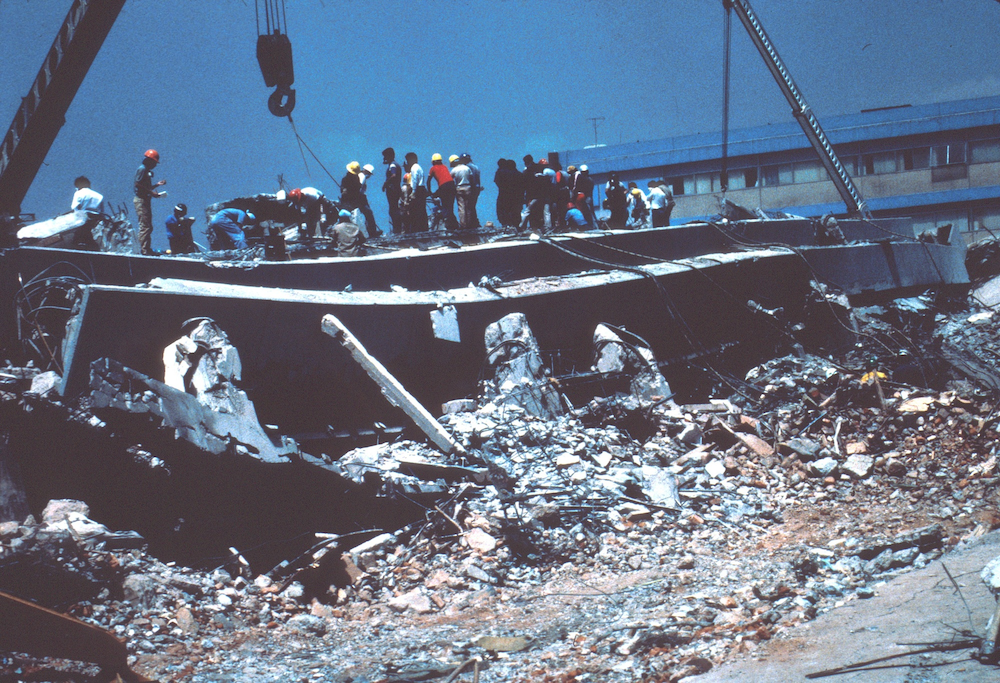
\includegraphics[width=0.8\textwidth]{figures/1985_Mexico_Earthquake_smaller.png}
\end{center}

Basic insight from Bernard et al. (1989)

\end{frame}
%%%%%%%%%%%%%%%%%
\begin{frame}

\begin{center}
\includegraphics<1>[width=0.6\textwidth]{figures/network-noedges}
\includegraphics<2>[width=0.6\textwidth]{figures/network-edges}
\includegraphics<3>[width=0.6\textwidth]{figures/network-edges-sample}
\includegraphics<4>[width=0.6\textwidth]{figures/network-edges-sample-ego}
\end{center}
\Large{
\begin{center}
\onslide<4>{$\hat{N}_H=\frac{2}{10} \times 30 = 6$}
\end{center}
}

\end{frame}
%%%%%%%%%%%%%%%%%
\begin{frame}

\begin{itemize}
\item Requires a random sample from the entire population 
\item Respondents are asked:
\begin{itemize}
\item How many people do you know who are drug injectors? 
\item How many women do you know that have given birth in the last 12 months?
\item How many people do you know who are middle school teachers?
\item $\ldots$
\item How many people do you know named Michael?
\end{itemize}
\item ``Know'' typically defined: you know them and they know you and have you been in contact with them over the past two years
\end{itemize}

\end{frame}
%%%%%%%%%%%%%%%%%
\begin{frame}

\begin{center}
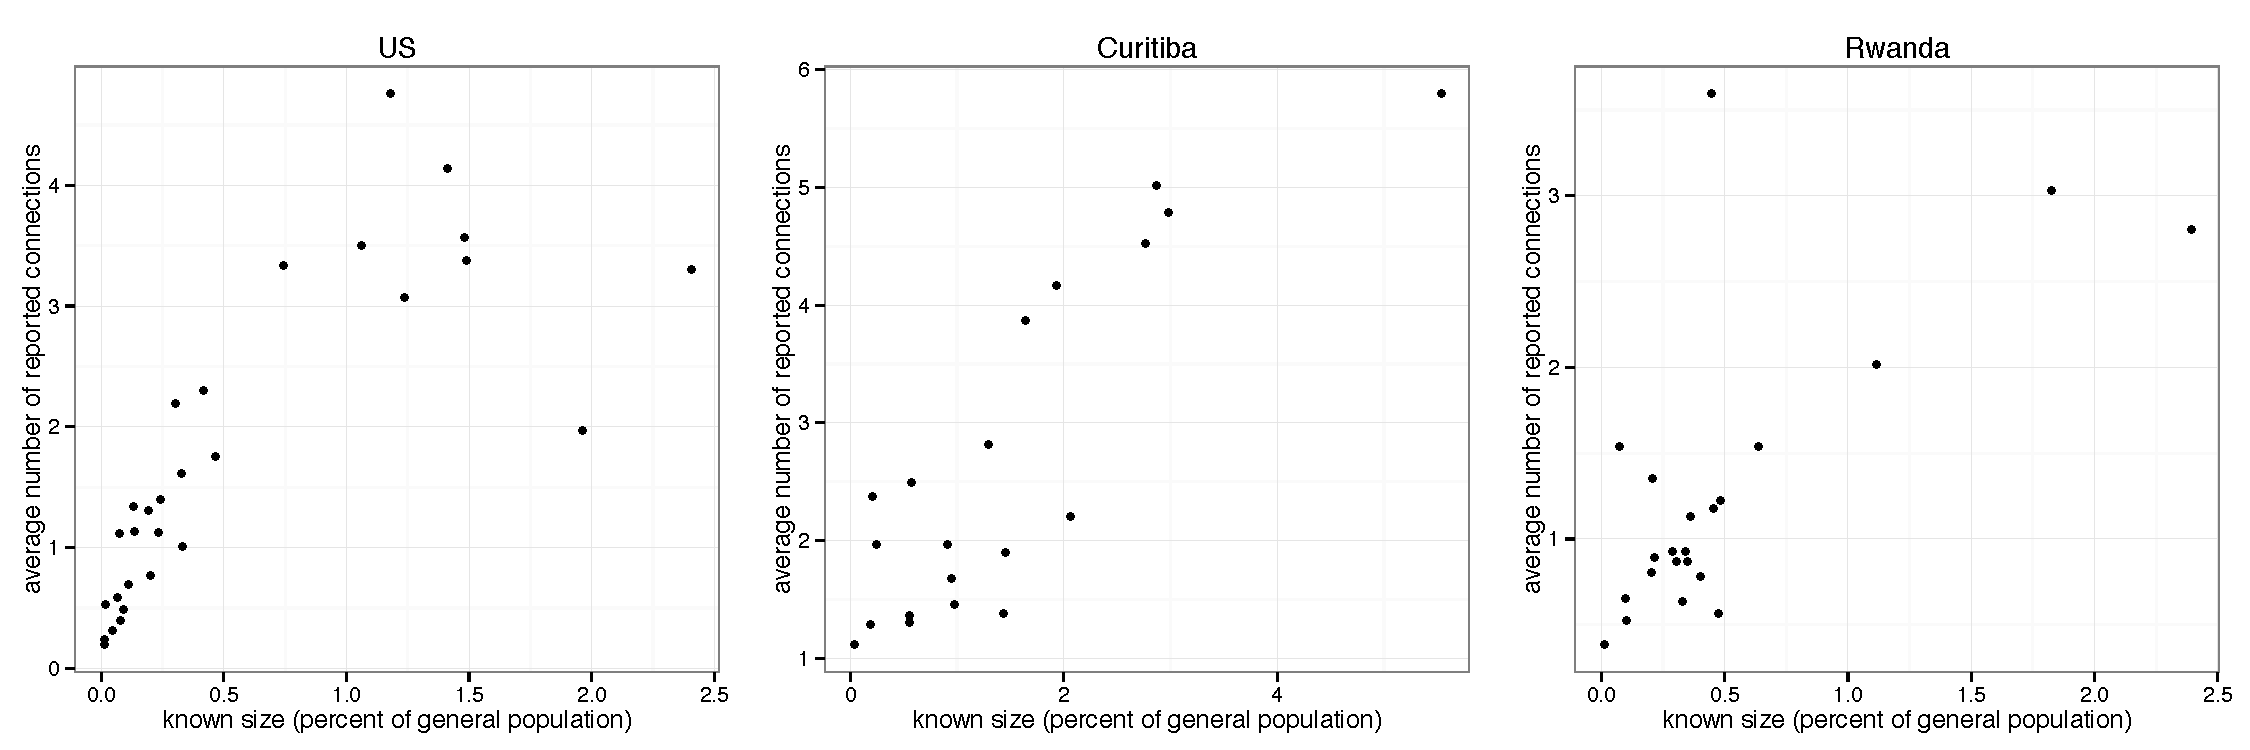
\includegraphics[width=0.95\textwidth]{figures/three_studies_truesize_known}
\end{center}
\vfill
On average, these answers are not crazy.

\end{frame}
%%%%%%%%%%%%%%%%%%
\begin{frame}

Other size estimation methods are problematic, and scale-up method has many nice properties:
\begin{itemize}
\item Requires a random sample of the general population, not specific contact with the hard-to-reach population \pause
\item Can be added as a module (5-10 minutes) in any existing survey \pause
\item Can estimate many target populations in a single survey \pause
\item Can be applied at the city-level, sub-national-level, or national-level \pause
\item Statistical methods are improvable \pause
\item Partially self-validating because it uses groups of known size
\end{itemize}

\end{frame}
%%%%%%%%%%%%%%%%%
\begin{frame}

\begin{figure}
  \centering
   \subfigure[United States]{
     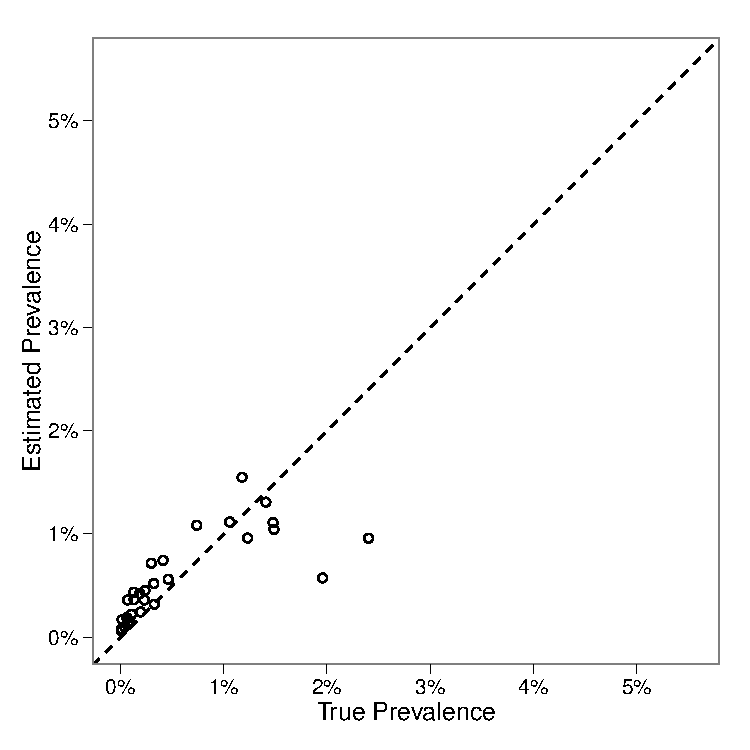
\includegraphics[width=0.3\textwidth]{figures/us-ivplot-forr01}}
  \hspace{0.0in}
    \subfigure[Curitiba]{
     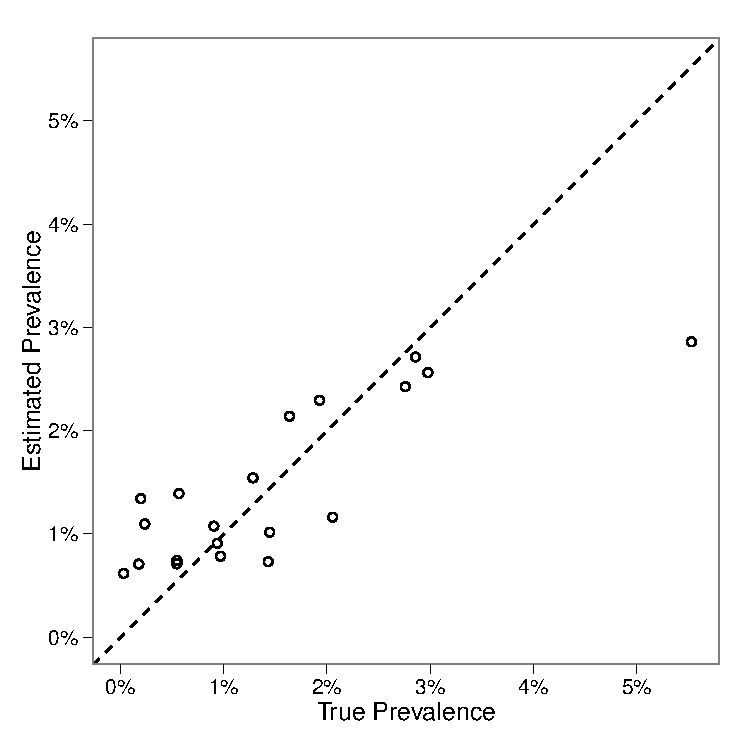
\includegraphics[width=0.3\textwidth]{figures/curitiba-ivplot-forr01}}     
  \hspace{0.0in}
    \subfigure[Rwanda]{
     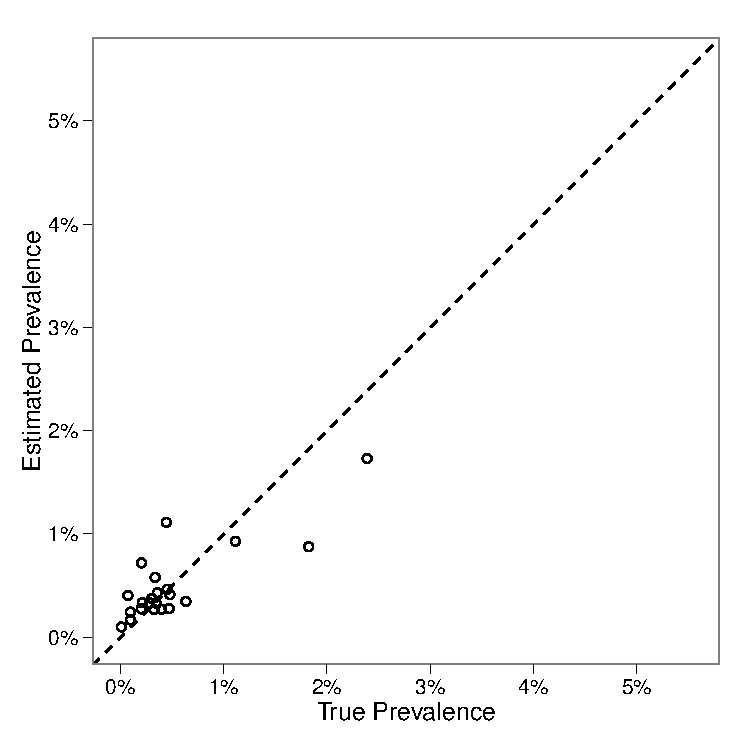
\includegraphics[width=0.3\textwidth]{figures/rwanda-ivplot-forr01}}     
\end{figure}

\end{frame}
%%%%%%%%%%%%%%%%
\begin{frame}

\LARGE{Network scale-up method, basic estimator}

\end{frame}
%%%%%%%%%%%%%%%%%%%%%%%%
\begin{frame}

\begin{equation*}
\hat{N}_H = \frac{\sum_i y_{i,H}}{\sum_i \hat{d}_i} \times N
\end{equation*}
\small{
\begin{itemize}
\item $\hat{N}_H$: number of people in the hidden population
\item $y_{i,H}$: number of people in hidden population known by person $i$
\item $\hat{d}_i$: estimated number of people known by person $i$
\item $N$: number of people in the population
\end{itemize}
}

\end{frame}
%%%%%%%%%%%%%%%%%
\begin{frame}

\begin{equation*}
\hat{d}_i =  \frac{\sum_k y_{i,k}}{\sum_k N_k} \times N
\end{equation*}
\small{
\begin{itemize}
\item $\hat{d}_i$: estimated number of people known by person $i$
\item $y_{i,k}$: number of people in group $k$ known by person $i$
\item $N_k$: number of people in group $k$
\item $N$: number of people in the population
\end{itemize}
}

\end{frame}
%%%%%%%%%%%%%%%%%
\begin{frame}

\begin{equation*}
\hat{d}_i = \frac{\sum_k y_{i,k}}{\sum_k N_k} \times N
\end{equation*}
\small{
\begin{itemize}
\item $\hat{d}_i$: estimated number of people known by person $i$
\item $y_{i,k}$: number of people in group $k$ known by person $i$
\item $N_k$: number of people in group $k$
\item $N$: number of people in the population
\end{itemize}
}

There are 50,000 Nsabimanas in Rwanda and 10 million people in Rwanda.  You know 2 Nsabimanas.  We estimate you know:
\pause
\begin{equation*}
\hat{d}_i = \frac{2}{50,000} \times 10 \mbox{ million} = 400 \mbox{ people} 
\end{equation*}

\end{frame}
%%%%%%%%%%%%%%%%
\begin{frame}

\begin{equation*}
\hat{d}_i = \frac{\sum_k  y_{i,k}}{\sum_k N_k} \times N
\end{equation*}
\small{
\begin{itemize}
\item $\hat{d}_i$: estimated number of people known by person $i$
\item $y_{i,k}$: number of people in group $k$ known by person $i$
\item $N_k$: number of people in group $k$
\item $N$: number of people in the population
\end{itemize}
}

There are 50,000 Nsabimanas in Rwanda; 1,000 Priests; and 10 million people in Rwanda.  You know 2 Nsabimanas and 1 priest.  We estimate you know:
\pause
\begin{equation*}
\hat{d}_i = \frac{2 + 1}{50,000 + 1,000} \times 10 \mbox{ million} \approx 600 \mbox{ people} 
\end{equation*}

\end{frame}
%%%%%%%%%%%%%%%%%%%%%%%%%%%%%%%%
\begin{frame}

\begin{equation*}
\hat{N}_H = \frac{\sum_i y_{i,H}}{\sum_i \hat{d}_i} \times N
\end{equation*}
\small{
\begin{itemize}
\item $\hat{N}_H$: number of people in the hidden population
\item $y_{i,H}$: number of people in hidden population known by person $i$
\item $\hat{d}_i$: estimated number of people known by person $i$
\item $N$: number of people in the population
\end{itemize}
}

\begin{itemize}
\item Person 1 knows 2 female sex workers and 400 people
\item Person 2 knows 4 female sex workers and 600 people
\end{itemize}
\pause
\begin{equation*}
\hat{N}_H  = \frac{2 + 4}{400 + 600} \times 10 \mbox{ million} = 60,000 \mbox{ people} 
\end{equation*}

\end{frame}
%%%%%%%%%%%%%%%%%
\begin{frame}

\begin{center}
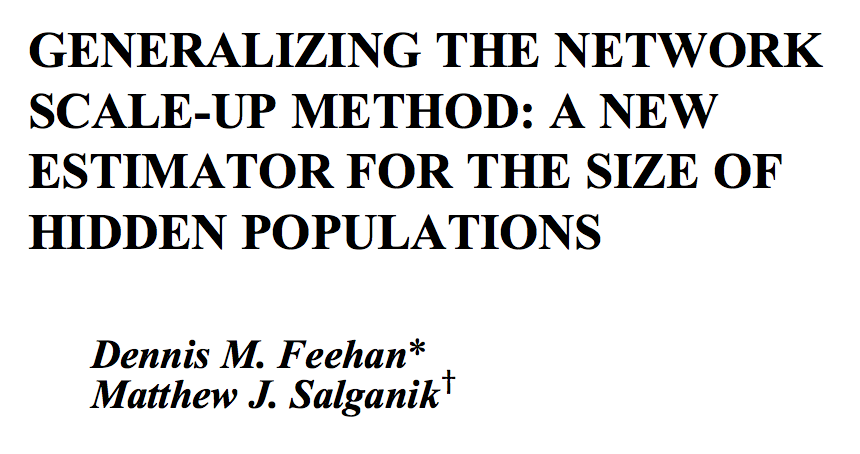
\includegraphics[width=0.5\textwidth]{figures/feehan_generalizing_2016_title}
\end{center}

\begin{itemize}
\item We develop the generalized scale-up estimator and use it to point out possible biases in basic scale-up estimator, but requires two data collections, which is rare (but wait until lecture 23) \pause
\item For the purposes of this class, focus on basic scale-up estimator and the correction factors needed for it
\end{itemize}

\end{frame}
%%%%%%%%%%%%%%%%%%%%%%%%%%%%%%%%%
\begin{frame}

\begin{center}
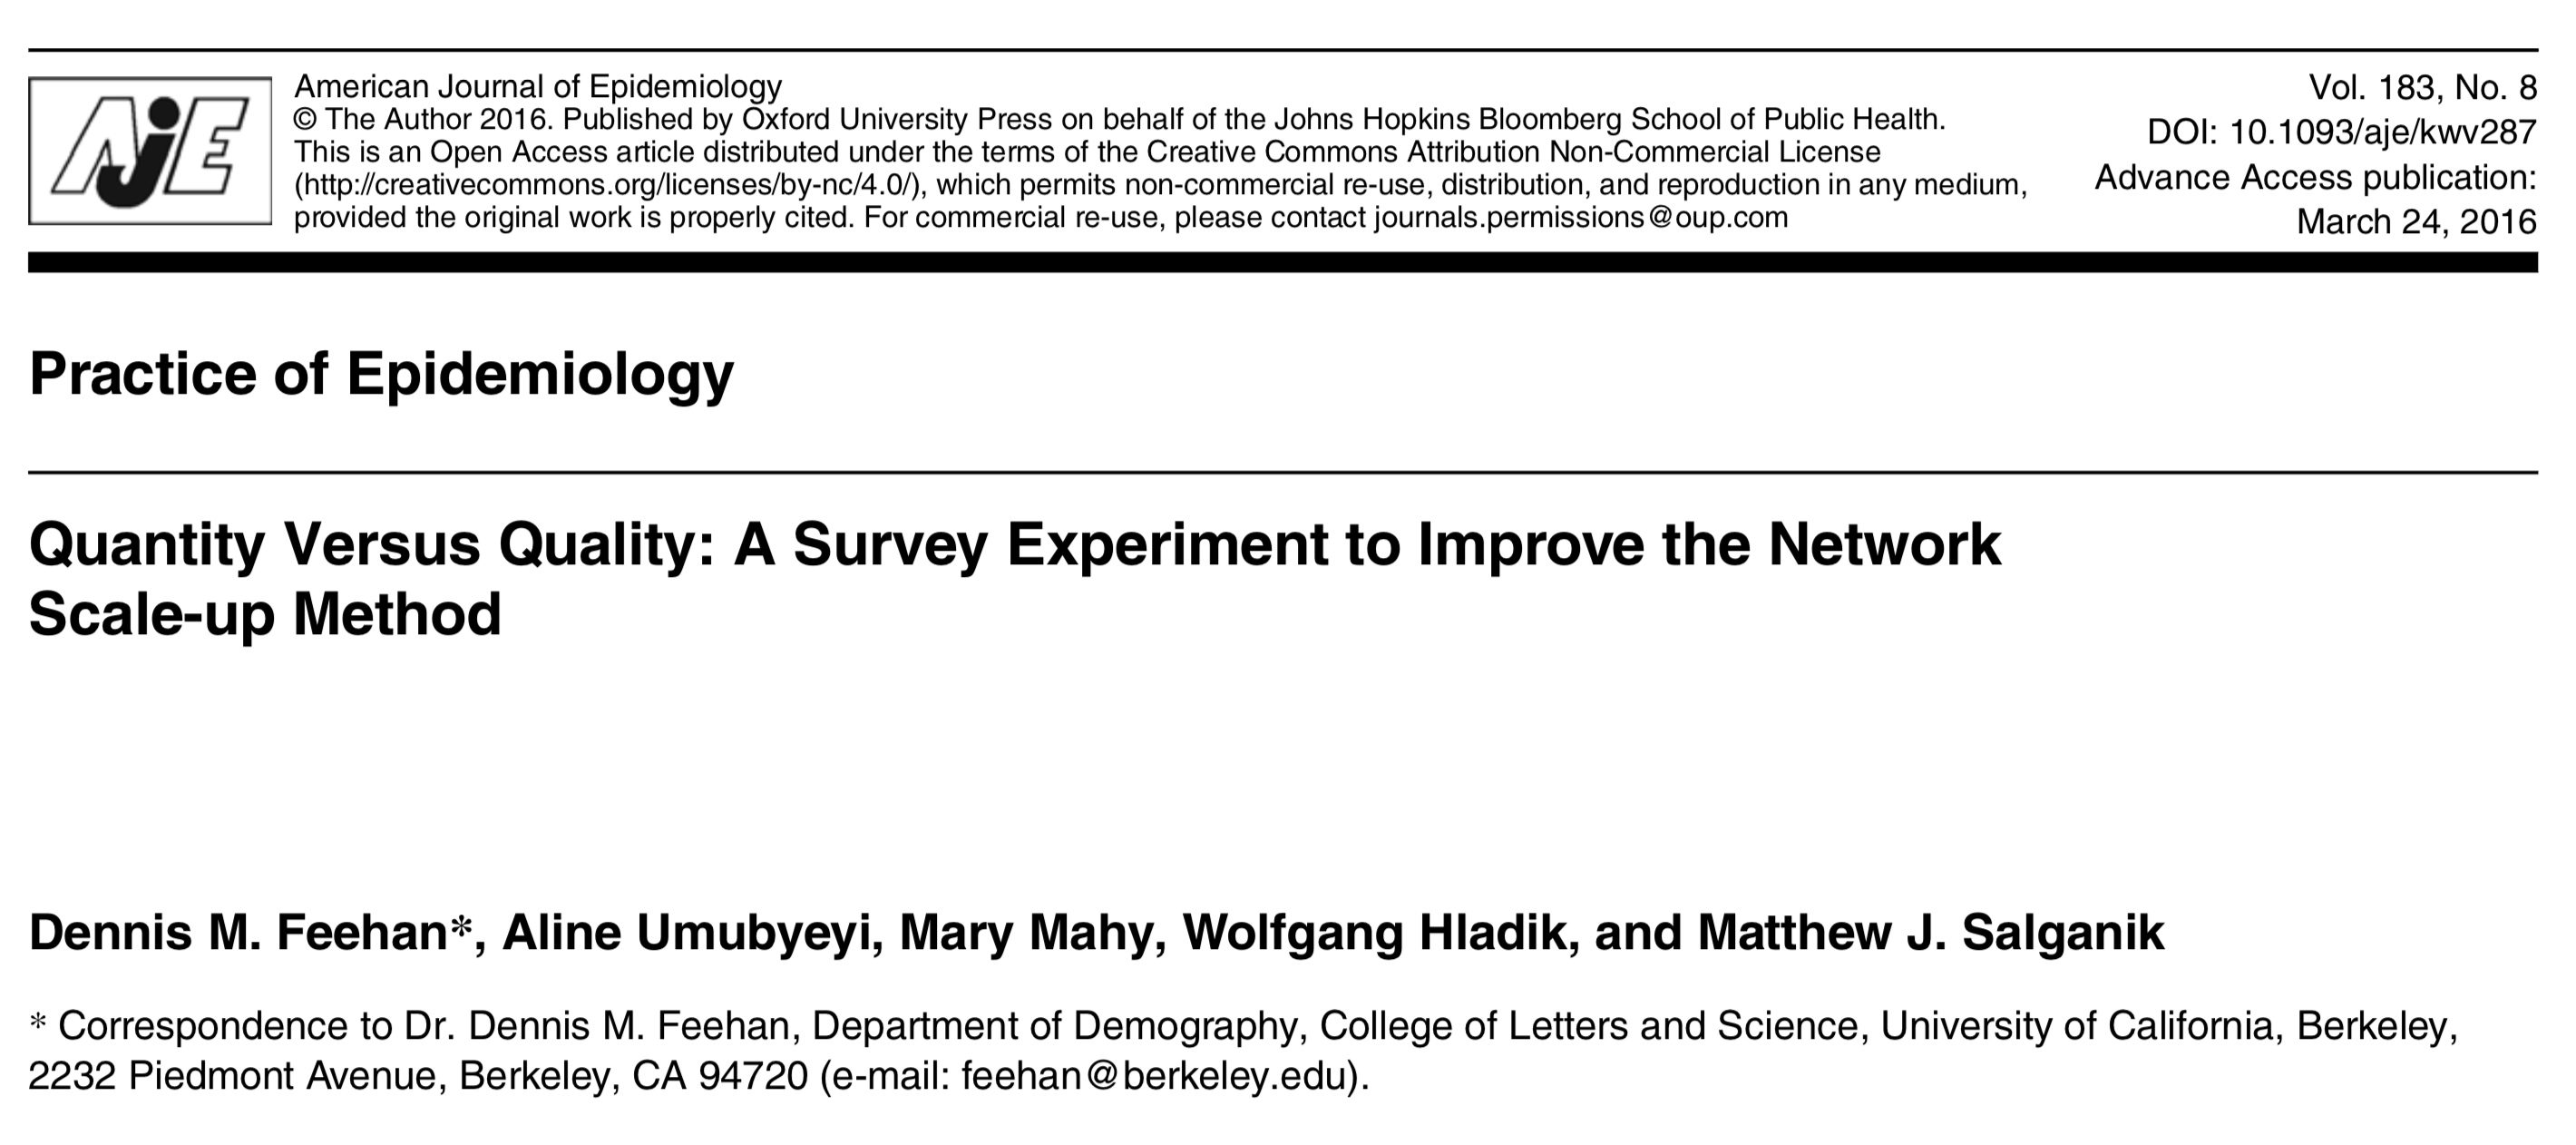
\includegraphics[width=0.5\textwidth]{figures/feehan_quantity_2016_title}
\end{center}

\begin{itemize}
\item Are there tie definitions other than ``to know'' that would lead to better estimates? We did a survey experiment to compare different definitions and then combined them to produce a single estimate \pause
\item Notice how we decided which is better and how we combined estimates \pause
\item Notice how we dealt with the many things we didd not know with sensitivity analysis. \pause
\end{itemize}

\end{frame}
%%%%%%%%%%%%%%%%%%%%%%%%%
\begin{frame}

{\Large
\begin{center}
Enjoy the reading
\end{center}
}

\end{frame}
%%%%%%%%%%%%%%%%%%%%%%%%%
% 1/2 Network scale-up method
%%%%%%%%%%%%%%%%%%%%%%%%
\begin{frame}

\LARGE{Network scale-up method}

\end{frame}
%%%%%%%%%%%%%%%%%%%%%%%%
\begin{frame}
\frametitle{}

\begin{center}
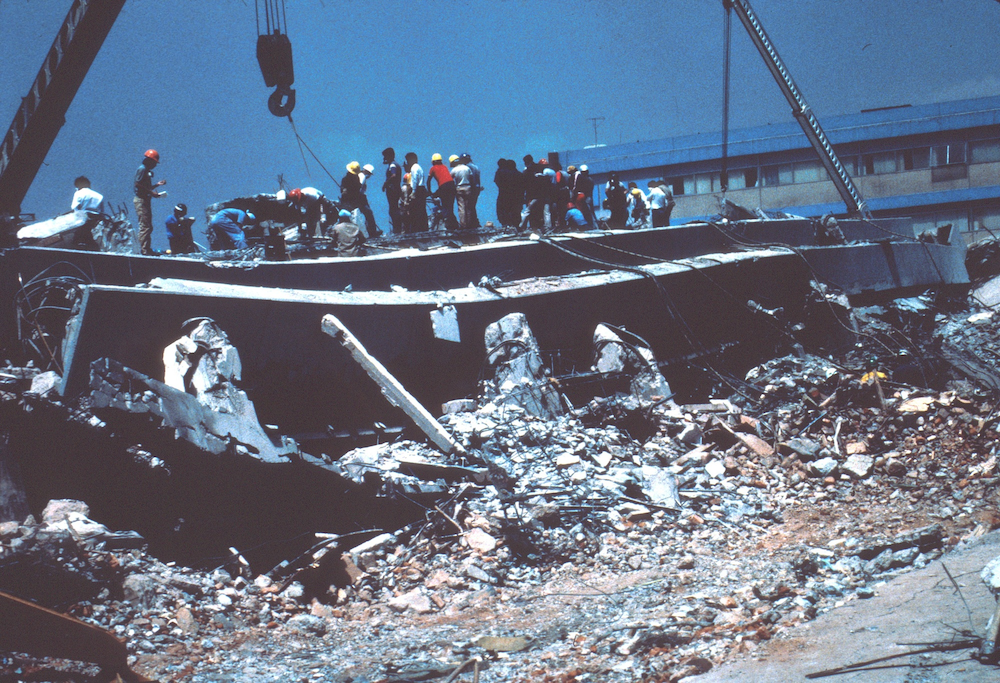
\includegraphics[width=0.8\textwidth]{figures/1985_Mexico_Earthquake_smaller.png}
\end{center}

Basic insight from Bernard et al. (1989)

\end{frame}
%%%%%%%%%%%%%%%%%
\begin{frame}

\begin{center}
\includegraphics<1>[width=0.6\textwidth]{figures/network-noedges}
\includegraphics<2>[width=0.6\textwidth]{figures/network-edges}
\includegraphics<3>[width=0.6\textwidth]{figures/network-edges-sample}
\includegraphics<4>[width=0.6\textwidth]{figures/network-edges-sample-ego}
\end{center}
\Large{
\begin{center}
\onslide<4>{$\hat{N}_H=\frac{2}{10} \times 30 = 6$}
\end{center}
}

\end{frame}
%%%%%%%%%%%%%%%%%
\begin{frame}

\begin{itemize}
\item Requires a random sample from the entire population 
\item Respondents are asked:
\begin{itemize}
\item How many people do you know who are drug injectors? 
\item How many women do you know that have given birth in the last 12 months?
\item How many people do you know who are middle school teachers?
\item $\ldots$
\item How many people do you know named Michael?
\end{itemize}
\item ``Know'' typically defined: you know them and they know you and have you been in contact with them over the past two years
\end{itemize}

\end{frame}
%%%%%%%%%%%%%%%%%
\begin{frame}

\begin{center}
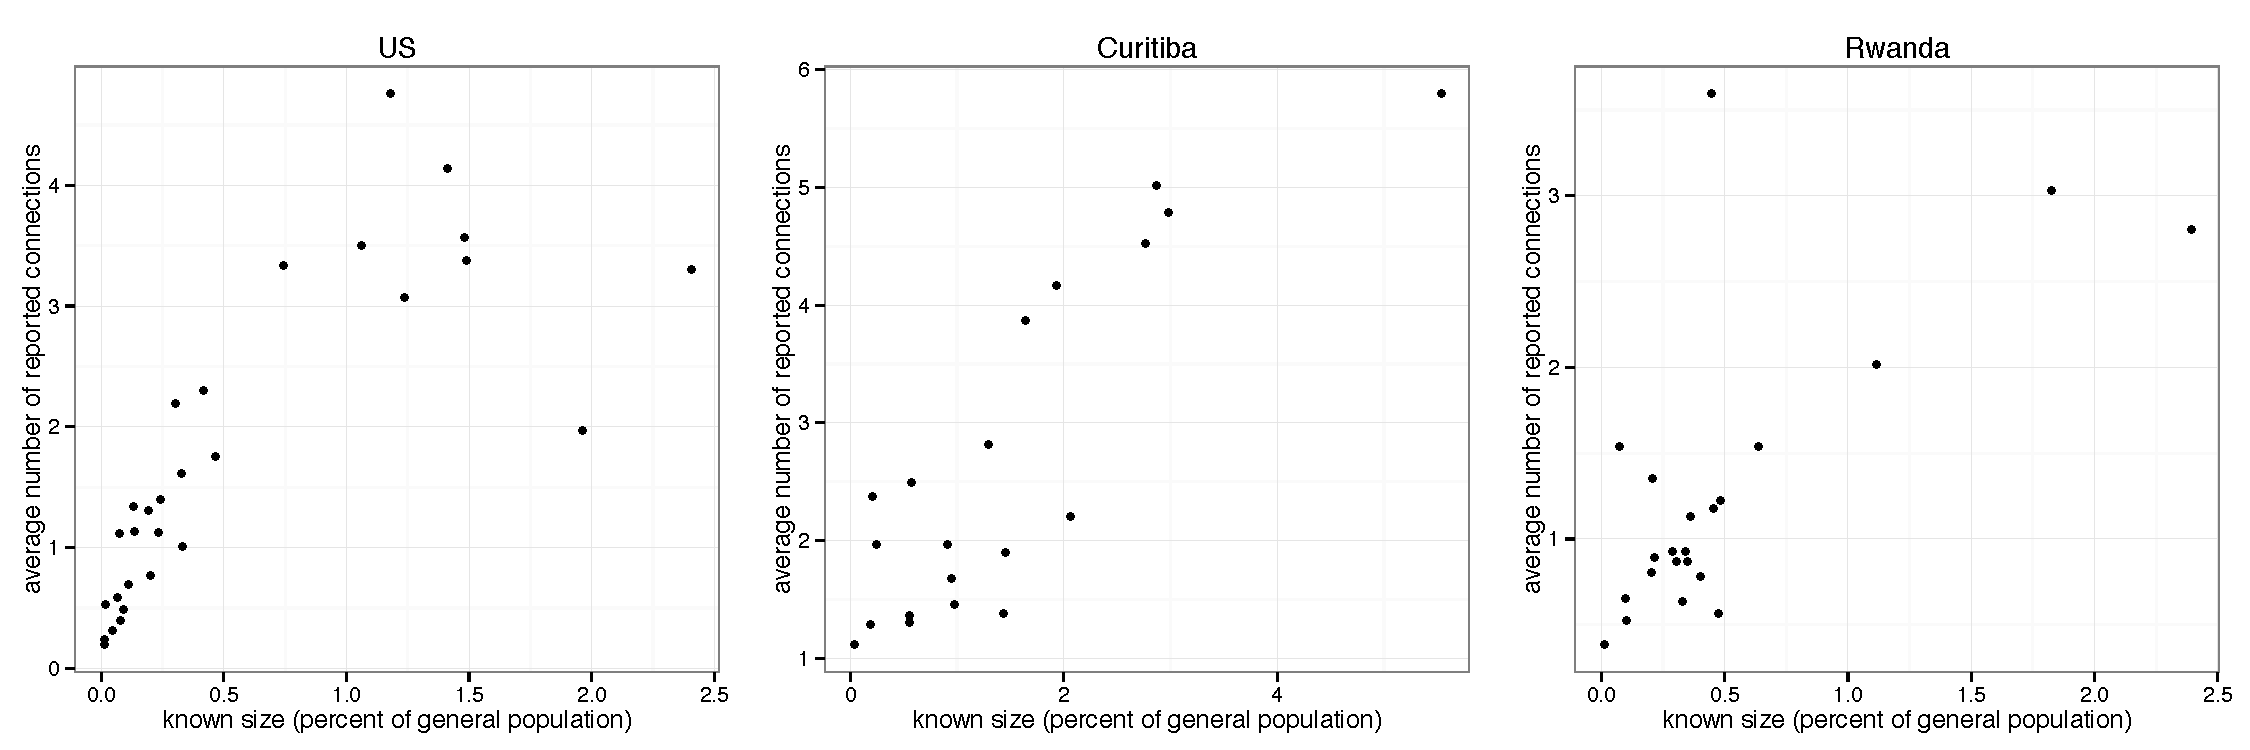
\includegraphics[width=0.95\textwidth]{figures/three_studies_truesize_known}
\end{center}
\vfill
On average, these answers are not crazy.

\end{frame}
%%%%%%%%%%%%%%%%%%
\begin{frame}

Other size estimation methods are problematic, and scale-up method has many nice properties:
\begin{itemize}
\item Requires a random sample of the general population, not specific contact with the hard-to-reach population 
\item Can be added as a module (5-10 minutes) in any existing survey 
\item Can estimate many target populations in a single survey 
\item Can be applied at the city-level, sub-national-level, or national-level
\item Statistical methods are improvable 
\item Partially self-validating because it uses groups of known size
\end{itemize}

\note{go quickly since they saw these in pre-read video}

\end{frame}
%%%%%%%%%%%%%%%%%
\begin{frame}

\begin{figure}
  \centering
   \subfigure[United States]{
     \label{fig:united_states} % Label for first subfigure
     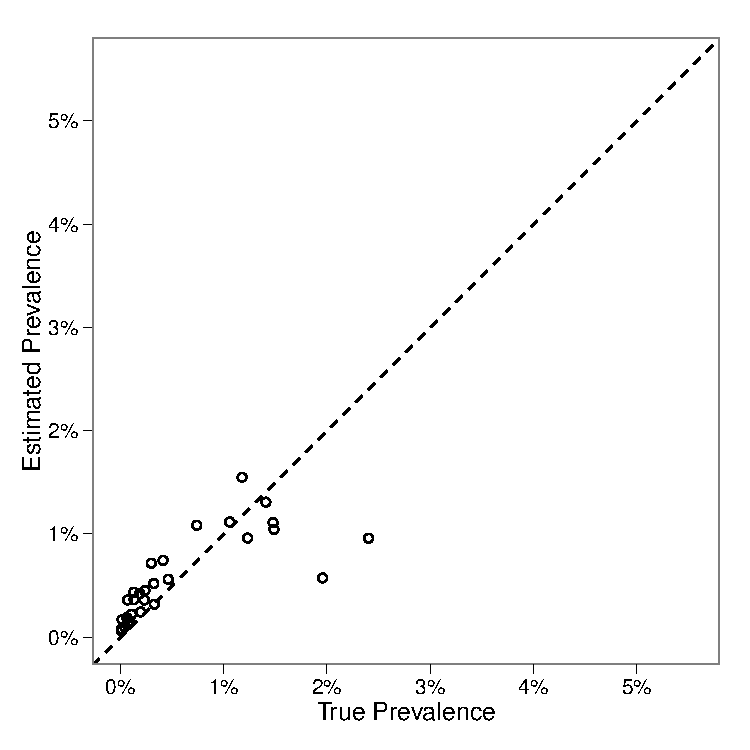
\includegraphics[width=0.3\textwidth]{figures/us-ivplot-forr01}}
  \hspace{0.0in}
    \subfigure[Curitiba]{
     \label{fig:curitiba} % Label for second subfigure
     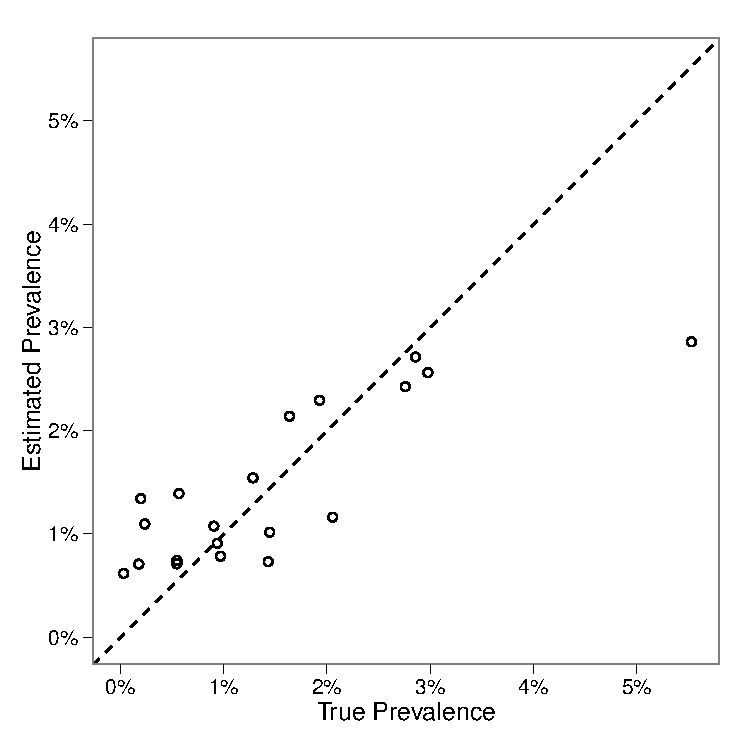
\includegraphics[width=0.3\textwidth]{figures/curitiba-ivplot-forr01}}     
  \hspace{0.0in}
    \subfigure[Rwanda]{
     \label{fig:rwanda} % Label for third subfigure
     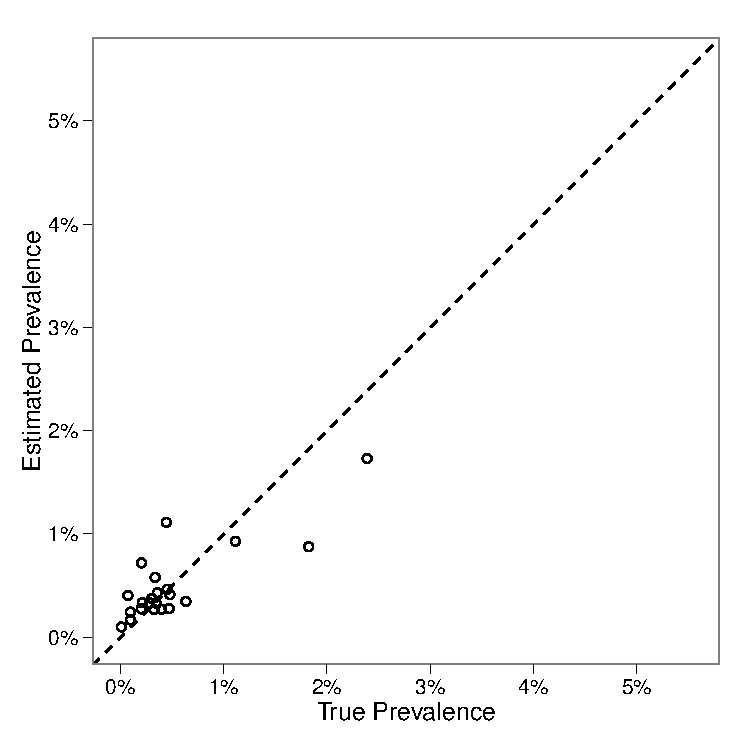
\includegraphics[width=0.3\textwidth]{figures/rwanda-ivplot-forr01}}     
\end{figure}

\end{frame}
%%%%%%%%%%%%%%%%
\begin{frame}

But, basic scale-up also has problems.  I will focus on insights about basic scale-up that we discovered from developing the generalized scale-up.

\end{frame}
%%%%%%%%%%%%%%%%%%%%%%%%%%%%%%%%%
\begin{frame}

\LARGE{Personal background}

\end{frame}
%%%%%%%%%%%%%%%%%%%%%%%%
\begin{frame}

How did I end up working on this research?\pause
\begin{itemize}
\item Working on sampling at the Census Bureau \pause
\item When I began grad school I knew about sampling and was interested in networks and Doug Heckathorn was working on respondent-driven sampling \pause
\item Respondent-driven sampling lead to the network scale-up method
\end{itemize}

\end{frame}
%%%%%%%%%%%%%%%%%%%%%%%%
\begin{frame}

\begin{columns}[t] % the "c" option specifies center vertical alignment

\column{0.45\textwidth} % column designated by a command
\begin{center}
{\Large Modeling}\\
counting with multiplicity
\end{center}

\column{0.10\textwidth}
\begin{center}
{\Large $\leftrightarrow$}
\end{center}

\column{0.40\textwidth}
\begin{center}
{\Large Empirical}\\
Rwanda (this lecture)\\
Brazil (next lecture) \\
\end{center}
\end{columns}

\end{frame}
%%%%%%%%%%%%%%%%%%%%%%%%%%%
\begin{frame}

If $\underbrace{y_{i,k} \sim Bin(d_i, N_k/N)}_\text{basic scale-up model}$, then maximum likelihood estimator is 

\begin{equation*}
\hat{N}_H = \frac{\sum_i y_{i,H}}{\sum_i \hat{d}_i} \times N
\end{equation*}
\small{
\begin{itemize}
\item $\hat{N}_H$: number of people in the hidden population
\item $y_{i,H}$: number of people in hidden population known by person $i$
\item $\hat{d}_i$: estimated number of people known by person $i$
\item $N$: number of people in the population
\end{itemize}
}
\vfill
See Killworth et al., (1998)
\end{frame}
%%%%%%%%%%%%%%%%%
\begin{frame}

\begin{center}
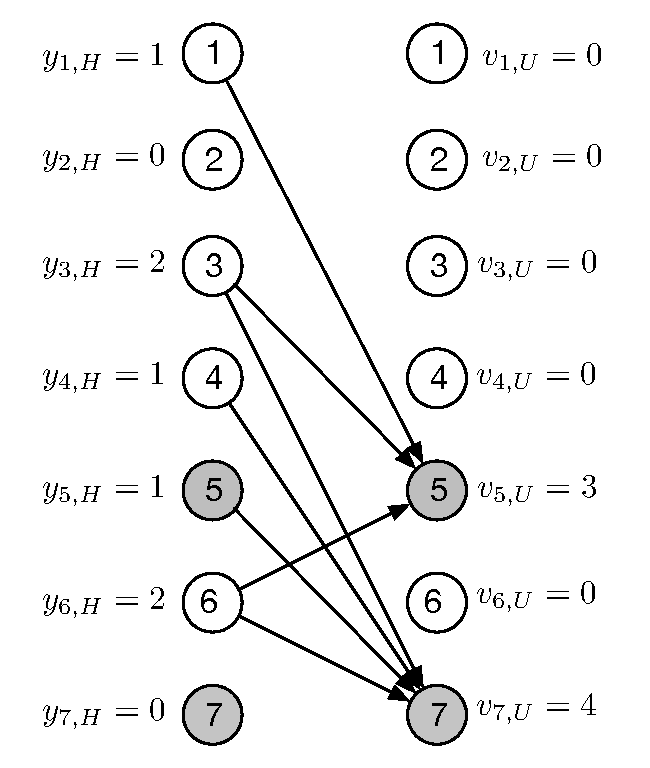
\includegraphics[height=0.8\textheight]{figures/reporting-network-panel2}
\end{center}

\end{frame}
%%%%%%%%%%%%%%%%%%
\begin{frame}

\begin{equation*}
\mbox{total out-reports} = \mbox{total in-reports}
\end{equation*}

\pause

\begin{align}
\mbox{total out-reports} & = \mbox{size of hidden pop}  \times  \nonumber \\ & \qquad \mbox{in-reports per member of hidden pop}  \nonumber
\end{align}

\pause 

\begin{equation*}
\mbox{size of hidden pop} = \frac{ \mbox{total out-reports} } { \mbox{in-reports per member of hidden pop} }
\end{equation*}

\end{frame}
%%%%%%%%%%%%%%%%%
\begin{frame}

\only<1>{
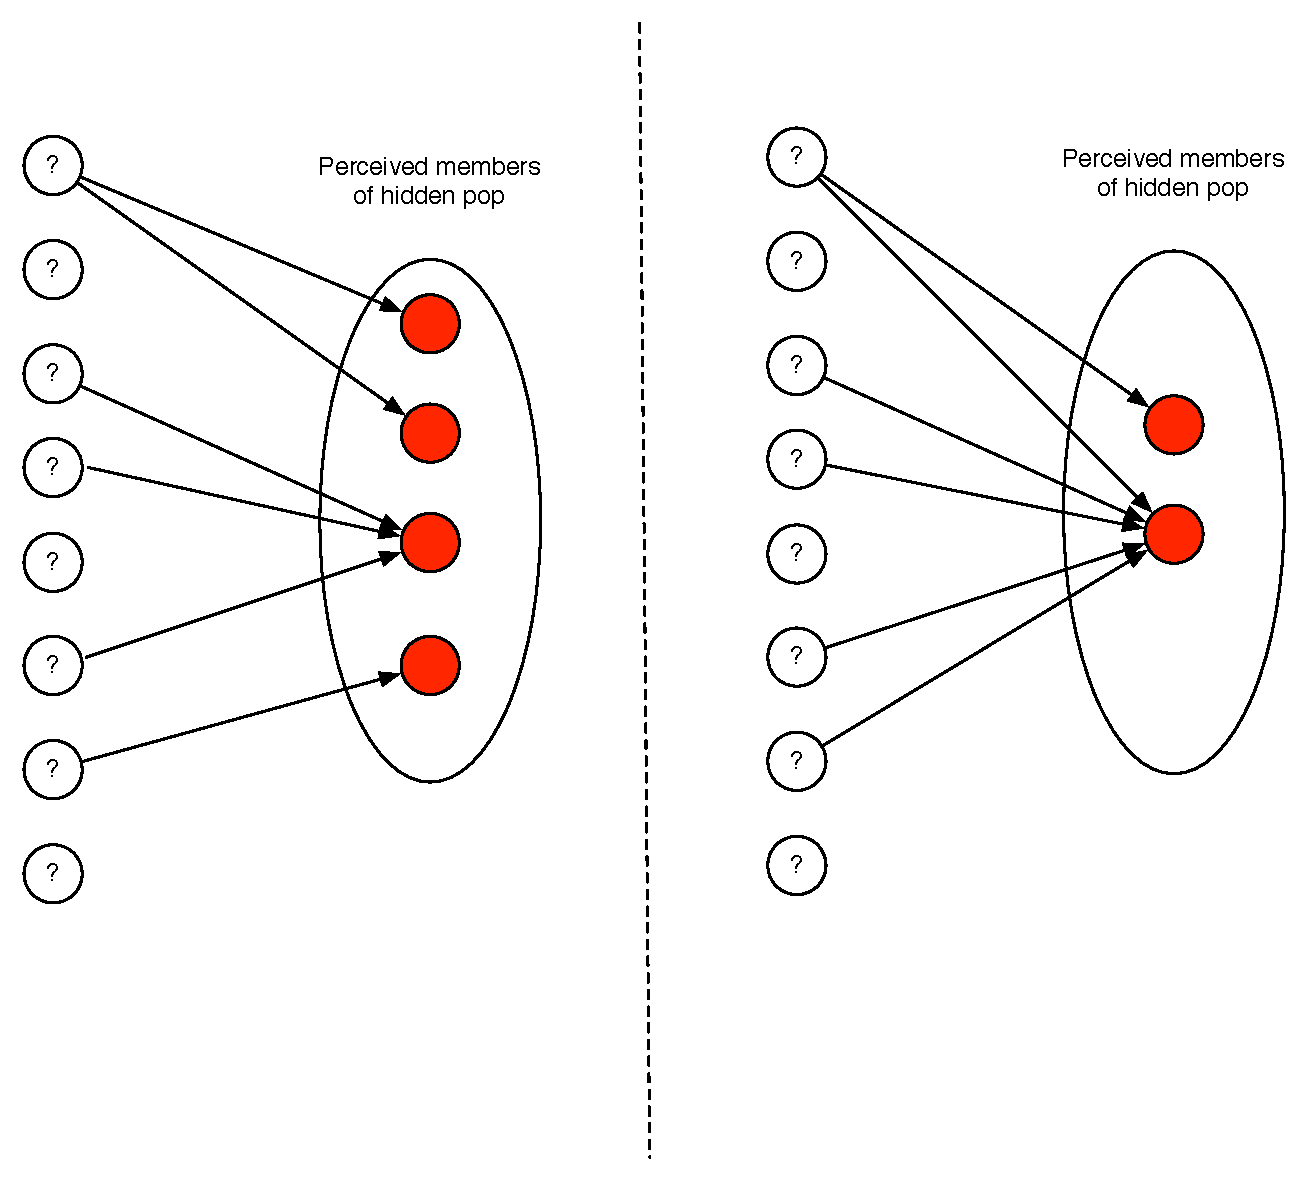
\includegraphics[width=0.8\textwidth]{figures/identification_problem_all}
}
\only<2>{
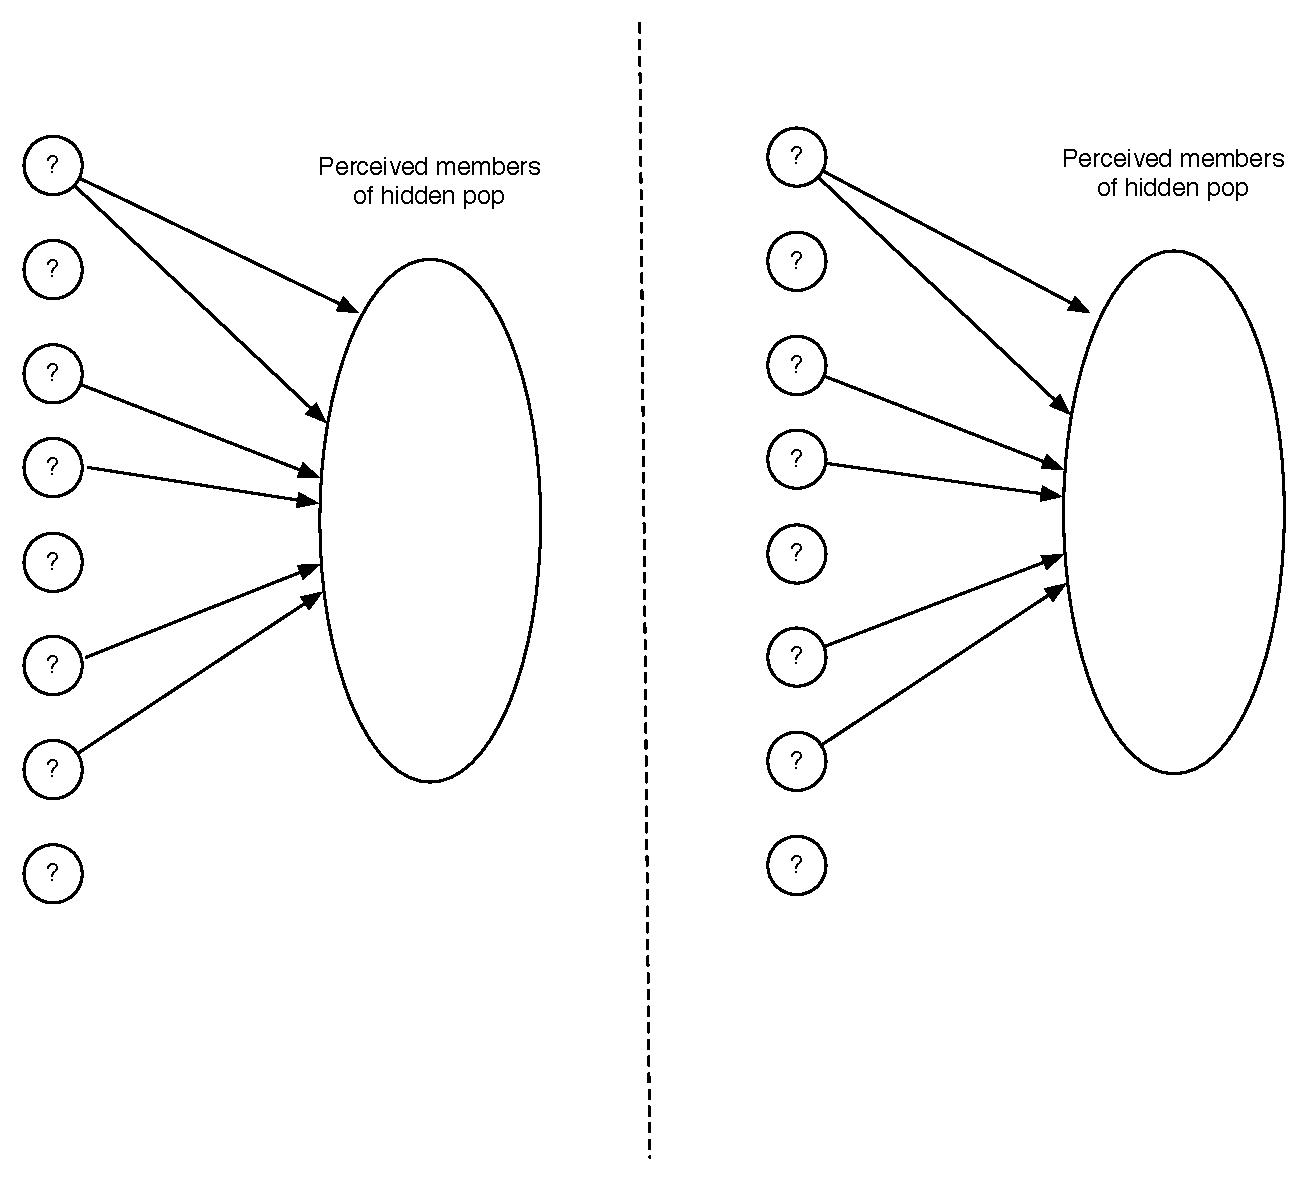
\includegraphics[width=0.8\textwidth]{figures/identification_problem_partial}
}
\end{frame}
%%%%%%%%%%%%%%%%%%
\begin{frame}

\begin{equation*}
\underbrace{N_H}_{\text{size of hidden pop}} = \frac{ \overbrace{ \sum_{i \in F} y_{i,H} }^{\text{total out-reports}} } { \underbrace{ \left( \sum_{i \in U} v_{i,F} / N_H \right) }_{\text{in-reports per member of hidden pop}} }
\end{equation*}
\pause
\vfill
If there are no false positives,
\begin{equation*}
\underbrace{N_H}_{\text{size of hidden pop}} = \frac{ \overbrace{ \sum_{i \in F} y_{i,H} }^{\text{total out-reports}} } { \underbrace{ \left( \sum_{\textcolor{blue}{i \in H}} v_{i,F} / N_H \right) }_{\text{avg visible degree of hidden pop}} }
\end{equation*}

\end{frame}
%%%%%%%%%%%%%%%%%
\begin{frame}

Generalized scale-up identity
\begin{equation*}
\underbrace{N_H}_{\text{size of hidden pop}} = \frac{ \overbrace{ \sum_{i \in F} y_{i,H} }^{\text{total out-reports}} } { \underbrace{ \left( \sum_{\textcolor{blue}{i \in H}} v_{i,F} / N_H \right) }_{\text{avg visible degree of hidden pop}} }
\end{equation*}

\vfill
Basic scale-up estimator
\only<1>{
\begin{equation*}
\hat{N}_H = \frac{\sum_{i \in s_F} y_{i,H}}{\sum_{i \in s_F} \hat{d}_i} \times N
\end{equation*}
}

\only<2>{
\begin{equation*}
\underbrace{\hat{N}_H}_{\text{est size of hidden pop}} = \frac{\overbrace{\sum_{i \in s_F} y_{i,H}}^\text{total out-reports}} {\underbrace{\sum_{i \in s_F} \hat{d}_{i, U} / N}_\text{avg degree of pop} }
\end{equation*}
}

\end{frame}
%%%%%%%%%%%%%%%%%%
\begin{frame}

Counting with multiplicity approach:
\begin{itemize}
\item no assumptions about the underlying social network
\item extends naturally to incomplete social awareness
\item extends naturally to incomplete frames
\item extends naturally to complex sample designs
\end{itemize}

\end{frame}
%%%%%%%%%%%%%%%%%%%%%%%%%%%
\begin{frame}

\begin{center}
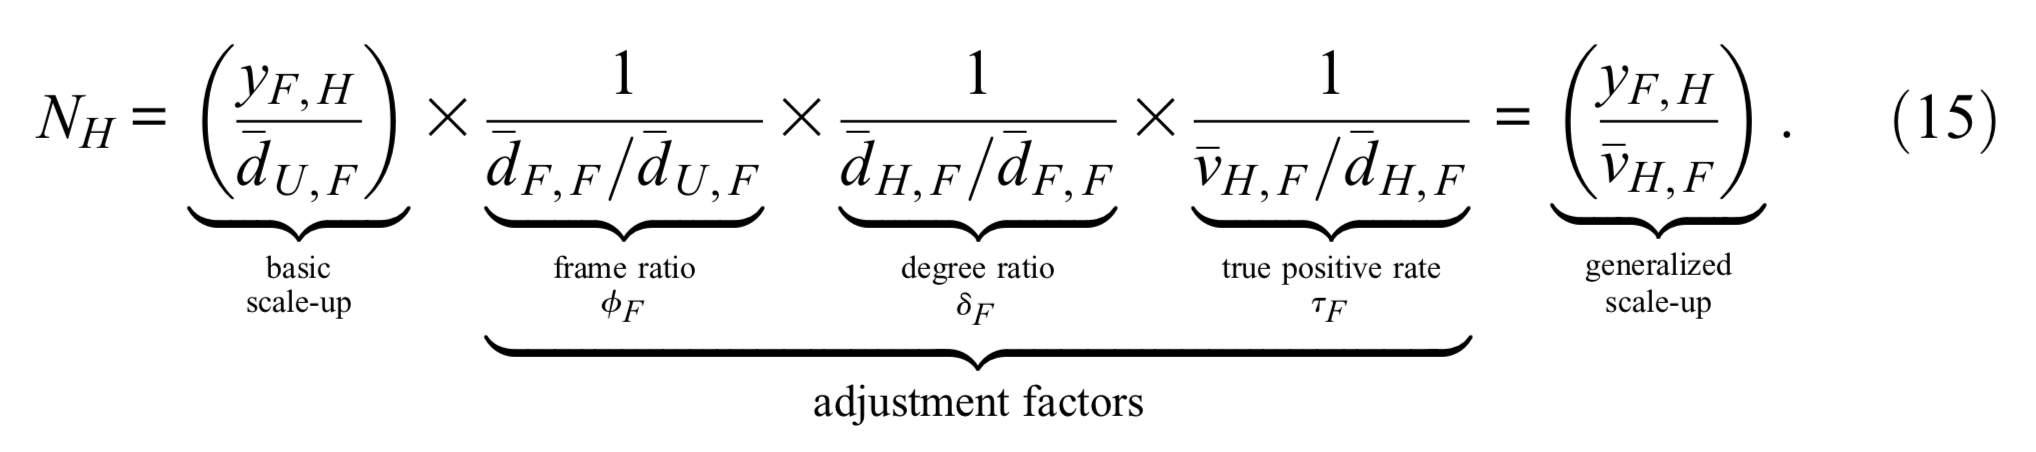
\includegraphics[width=0.95\textwidth]{figures/feehan_generalizing_2016_eq15}
\end{center}

\end{frame}
%%%%%%%%%%%%%%%%%%%%%%%%%%%%%
\begin{frame}

Frame ratio: Less a focus for us.  As a first approximation, sampling frame is adults you don't want to include kids in any of the reports

\end{frame}
%%%%%%%%%%%%%%%%%%%%%%%%%%%%
\begin{frame}

Degree ratio: If the hidden population has smaller network sizes than the general population, the size of the hidden population will be underestimated.  Likewise, if the hidden population has larger network sizes than the general population, the size of the hidden population will be overestimated.

\end{frame}
%%%%%%%%%%%%%%%%%%%%%%%%%%%%
\begin{frame}

Set of egos can be different from set of alters.
\vfill
\begin{columns}[c]
\column{0.3\textwidth}
\framebox{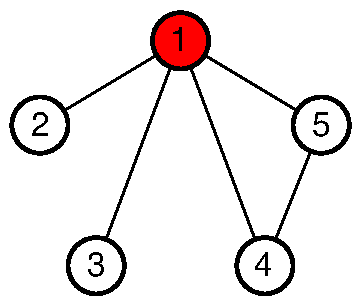
\includegraphics[height=0.8in]{figures/folded_network_slides}}
\phantom{1234}$p=0.2$
\column{0.6\textwidth}
\pause
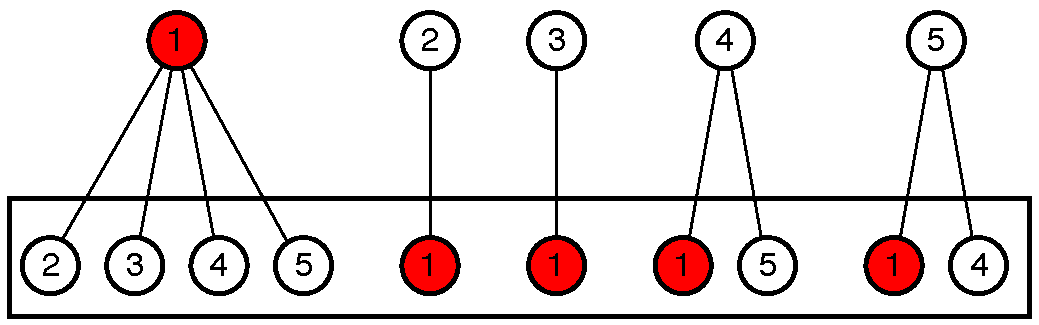
\includegraphics[height=0.8in]{figures/unfolded_network_slides}
\phantom{123456789123456789101112}
\phantom{1234567891234}$p_{alter}=0.4$
\end{columns}
\vfill
\pause
\begin{equation*}
p_{alter}=p \times \frac{\mbox{avg. degree (hidden pop.)}}{\mbox{avg. degree (general pop.)}}=p \delta
\end{equation*}
\vfill
Estimates will be biased by a factor of $\delta_F$ (``degree ratio'')

\end{frame}
%%%%%%%%%%%%%%%%%%
\begin{frame}

True positive rate: If people are connected to people in the hidden population but not aware of it, the size of the hidden population will be underestimated 

\end{frame}
%%%%%%%%%%%%%%%%%%%%%%%%%%%%
\begin{frame}

How might imperfect knowledge impact scale-up estimates?\\
Ego is not aware of everything about all of their alters.
\begin{center}
\includegraphics<1>[width=0.7\textwidth]{figures/network-edges-sample-ego-noinfotxerror}
\includegraphics<2>[width=0.7\textwidth]{figures/network-edges-sample-ego-infotxerror-formatt}
\end{center}
\pause
\vfill
Estimates will be biased by a factor of $\tau_F$ (``true positive rate'')

\vfill
More about this in next lecture 

\end{frame}
%%%%%%%%%%%%%%%%%%
\begin{frame}

\begin{center}
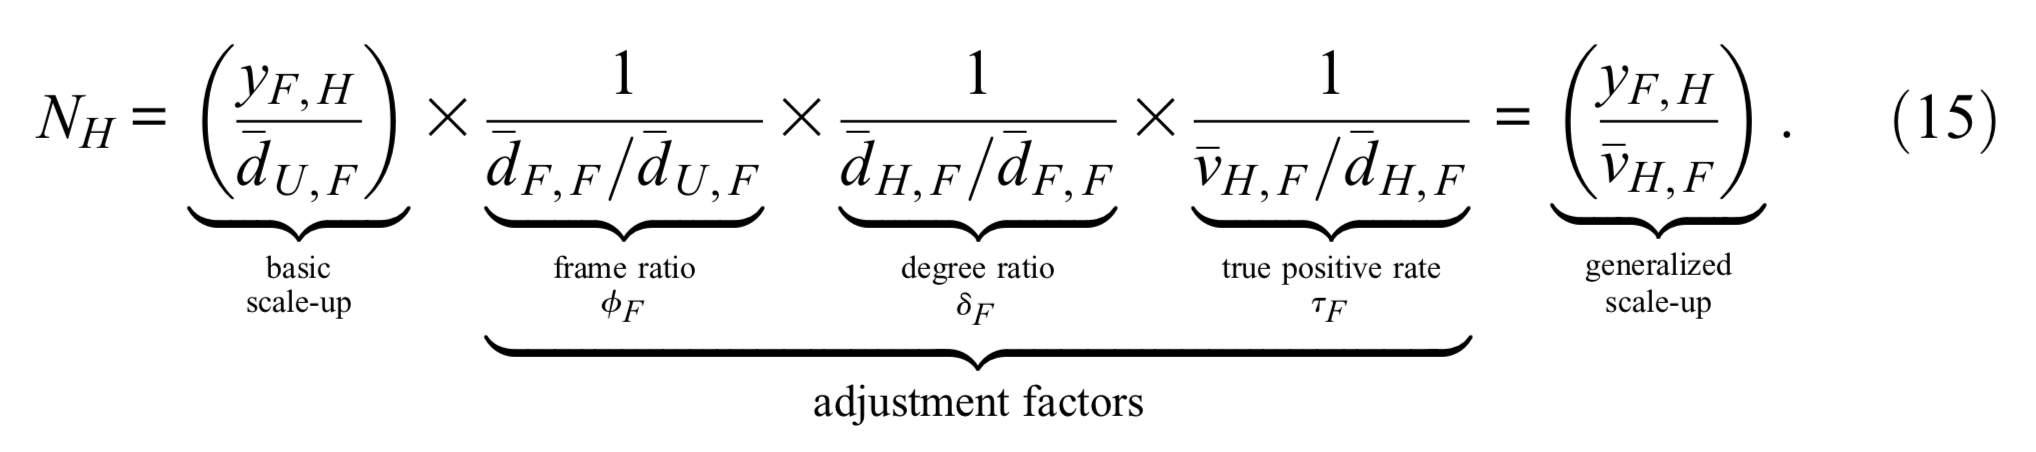
\includegraphics[width=0.95\textwidth]{figures/feehan_generalizing_2016_eq15}
\end{center}
 
\end{frame}
%%%%%%%%%%%%%%%%%%%%%%%%
\begin{frame}
\frametitle{From a talk I gave at a UNAIDS workshop}

Generalized scale-up approach
\begin{itemize}
\item simple estimators (just addition, subtraction, multiplication, and division)
\item handles incomplete social awareness
\item no assumptions about the underlying social network
\item handles incomplete frames
\item handles complex sample designs
\end{itemize}

\vfill
and could still be very wrong in practice!

\end{frame}
%%%%%%%%%%%%%%%%%%%%%%%%%
\begin{frame}

\begin{center}

\includegraphics[width=0.5\textwidth]{figures/slippery-when-wet}
\end{center}

\end{frame}
%%%%%%%%%%%%
\begin{frame}

Assumptions can be put into four broad categories
\begin{itemize}
\item sampling
\item social network structure
\item reporting
\item survey construction
\end{itemize}

\end{frame}
%%%%%%%%%%%
\begin{frame}

Results for non-sampling assumptions have this form:
\begin{center}
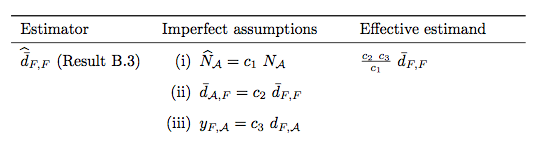
\includegraphics[width=0.7\textwidth]{figures/feehan_estimating_2014_tabd1_result1}
\end{center}

\end{frame}
%%%%%%%%%%%%
\begin{frame}

\begin{center}
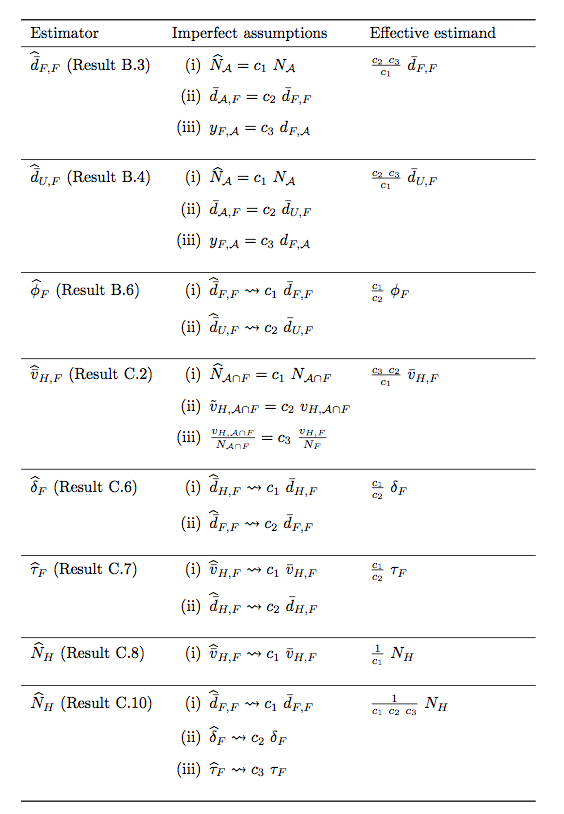
\includegraphics[height=\textheight]{figures/feehan_estimating_2014_tabd1}
\end{center}

\end{frame}
%%%%%%%%%%%%%
\begin{frame}

\begin{center}

\includegraphics[width=0.3\textwidth]{figures/slippery-when-wet}
\end{center}

Fails when:
\begin{itemize}
\item adjustment factors not measured
\item adjustment factors measured poorly
\item reporting not consistent with awareness
\item variance estimation fails
\item  . . . .
\end{itemize}

\end{frame}
%%%%%%%%%%%%%%%%%%%%%%%%%%%%%%%
\begin{frame}

\begin{columns}[t] % the "c" option specifies center vertical alignment

\column{0.45\textwidth} % column designated by a command
\begin{center}
{\Large Modeling}\\
counting with multiplicity
\end{center}

\column{0.10\textwidth}
\begin{center}
{\Large $\leftrightarrow$}
\end{center}

\column{0.40\textwidth}
\begin{center}
{\Large Empirical}\\
Rwanda (this lecture)\\
Brazil (next lecture) \\
\end{center}
\end{columns}

\end{frame}
%%%%%%%%%%%%%%%%%%%%%%%%%%%%%%%%%%%%
% 2/2 Survey experiment with blending: A network scale-up study in Rwanda
%%%%%%%%%%%%%%%%%%%%%%%%%%%%%%%%%
\begin{frame}

\Large{
\begin{center}
How can we improve\\if we don't know how we are doing?
\end{center}
}

\end{frame}
%%%%%%%%%%%%%%%%%%%%%%%%%%%
\begin{frame}

\begin{center}
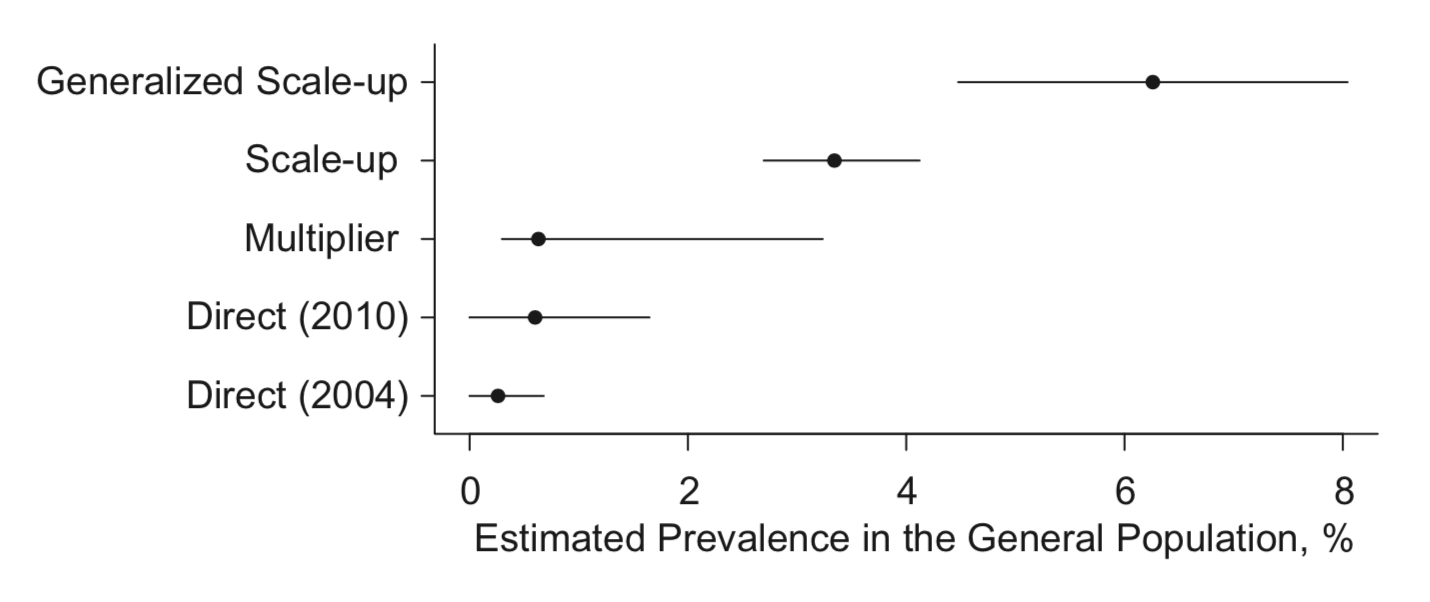
\includegraphics[width=0.9\textwidth]{figures/salganik_assessing_2011_fig2}
\end{center}
\small{
Source: Salganik, M.J., Fazito, D., Bertoni, N., Abdo, A.H., Mello, M.B., and Bastos, F.I. (2011)  \textit{American Journal of Epidemiology}. }

\end{frame}
%%%%%%%%%%%%%%%%%%%%%%%%%%%
\begin{frame}

\begin{center}
How can we reliably make progress in our ability to estimate quantities that will never be known?
\end{center}
\pause
\begin{itemize}
\item Theoretical 
\item Empirical 
\end{itemize}

\note{Theoretical include modeling like we saw in last video}

\end{frame}
%%%%%%%%%%%%%%%%%%%%%%%%%%%
\begin{frame}

\LARGE{Network scale-up study in Rwanda}

\end{frame}
%%%%%%%%%%%%%%%%%%%%%%%%%%%%%%%
\begin{frame}

Study in Rwanda was designed to estimate the number of 
\begin{itemize}
\item men who have sex with men
\item female sex workers
\item clients of female sex workers
\item injection drug users
\end{itemize}

\vfill
AND \\
\vfill
to produce generalizable knowledge about the scale-up method

\end{frame}
%%%%%%%%%%%%%%%%%
\begin{frame}

\begin{center}
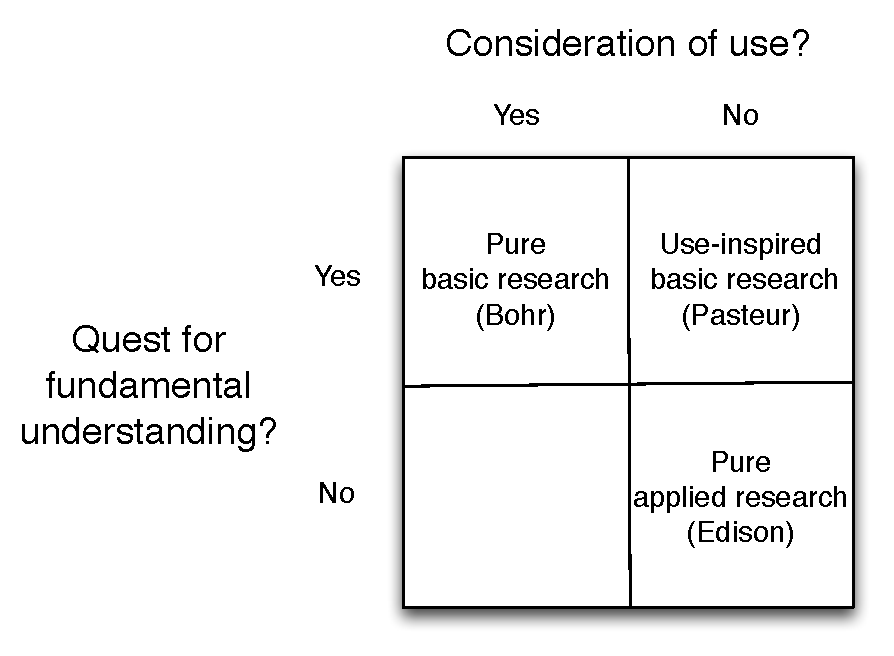
\includegraphics[width=0.6\textwidth]{figures/pasteurs_quadrant}
\end{center}

\end{frame}
%%%%%%%%%%%%%%%%%
\begin{frame}

\begin{itemize}
\item Why was UNAIDS excited about this study?
\pause
\item Why was the Rwandan National AIDS program excited about this study?
\pause
\item Why was I excited about this study?
\end{itemize}

\note{
UNAIDS: methods to be standardized around the world
Rwanda: chance to do more research and learn new methods
Me: advance scale-up and develop template for global use, also inspired by my time at tech companies
}

\end{frame}
%%%%%%%%%%%%%%%%%%%%%%%%%
\begin{frame}

\begin{center}
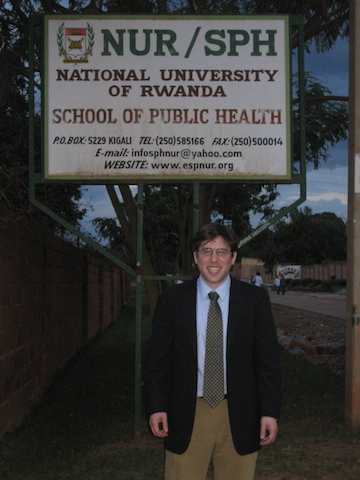
\includegraphics[height=0.9\textheight]{figures/rwanda_matt_nur.jpg}
\end{center}

\end{frame}
%%%%%%%%%%%%%%%%%%%%%%%%%%%%%%
\begin{frame}

\begin{center}
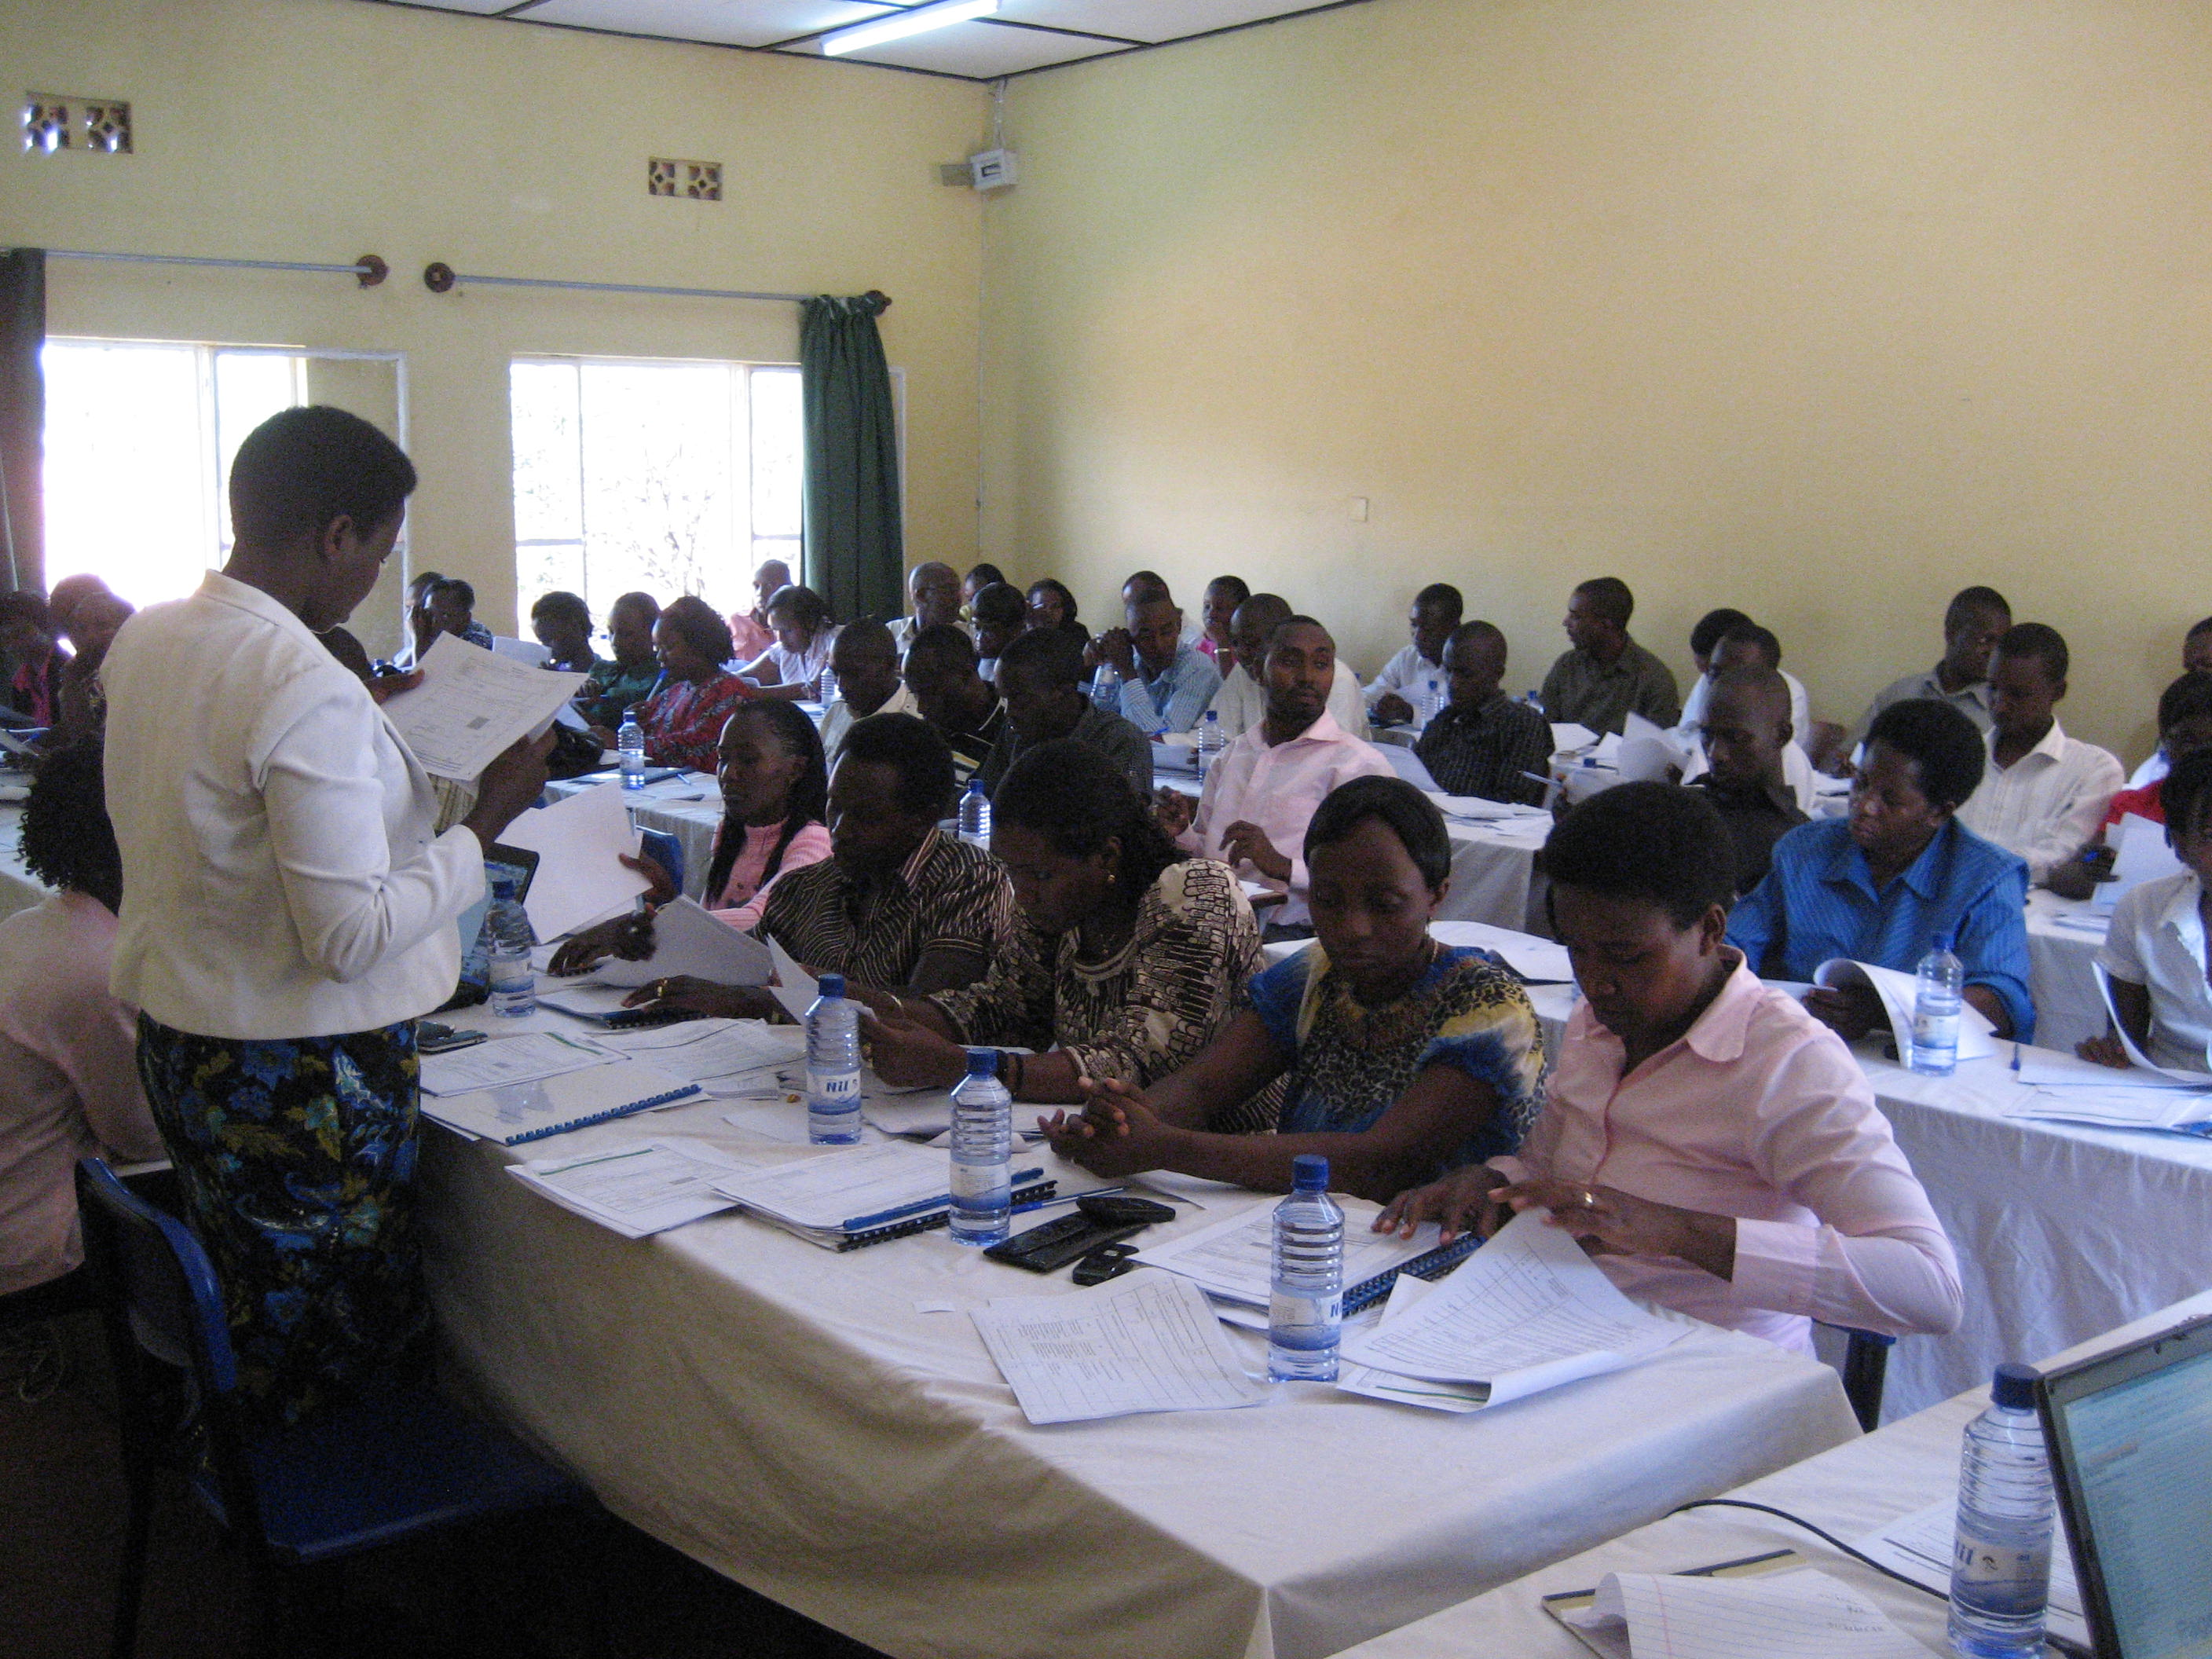
\includegraphics[width=0.8\textwidth]{figures/rwanda_interviewer_class.jpg}
\end{center}

\end{frame}
%%%%%%%%%%%%%%%%%%%%%%%%%%%
\begin{frame}

\begin{center}
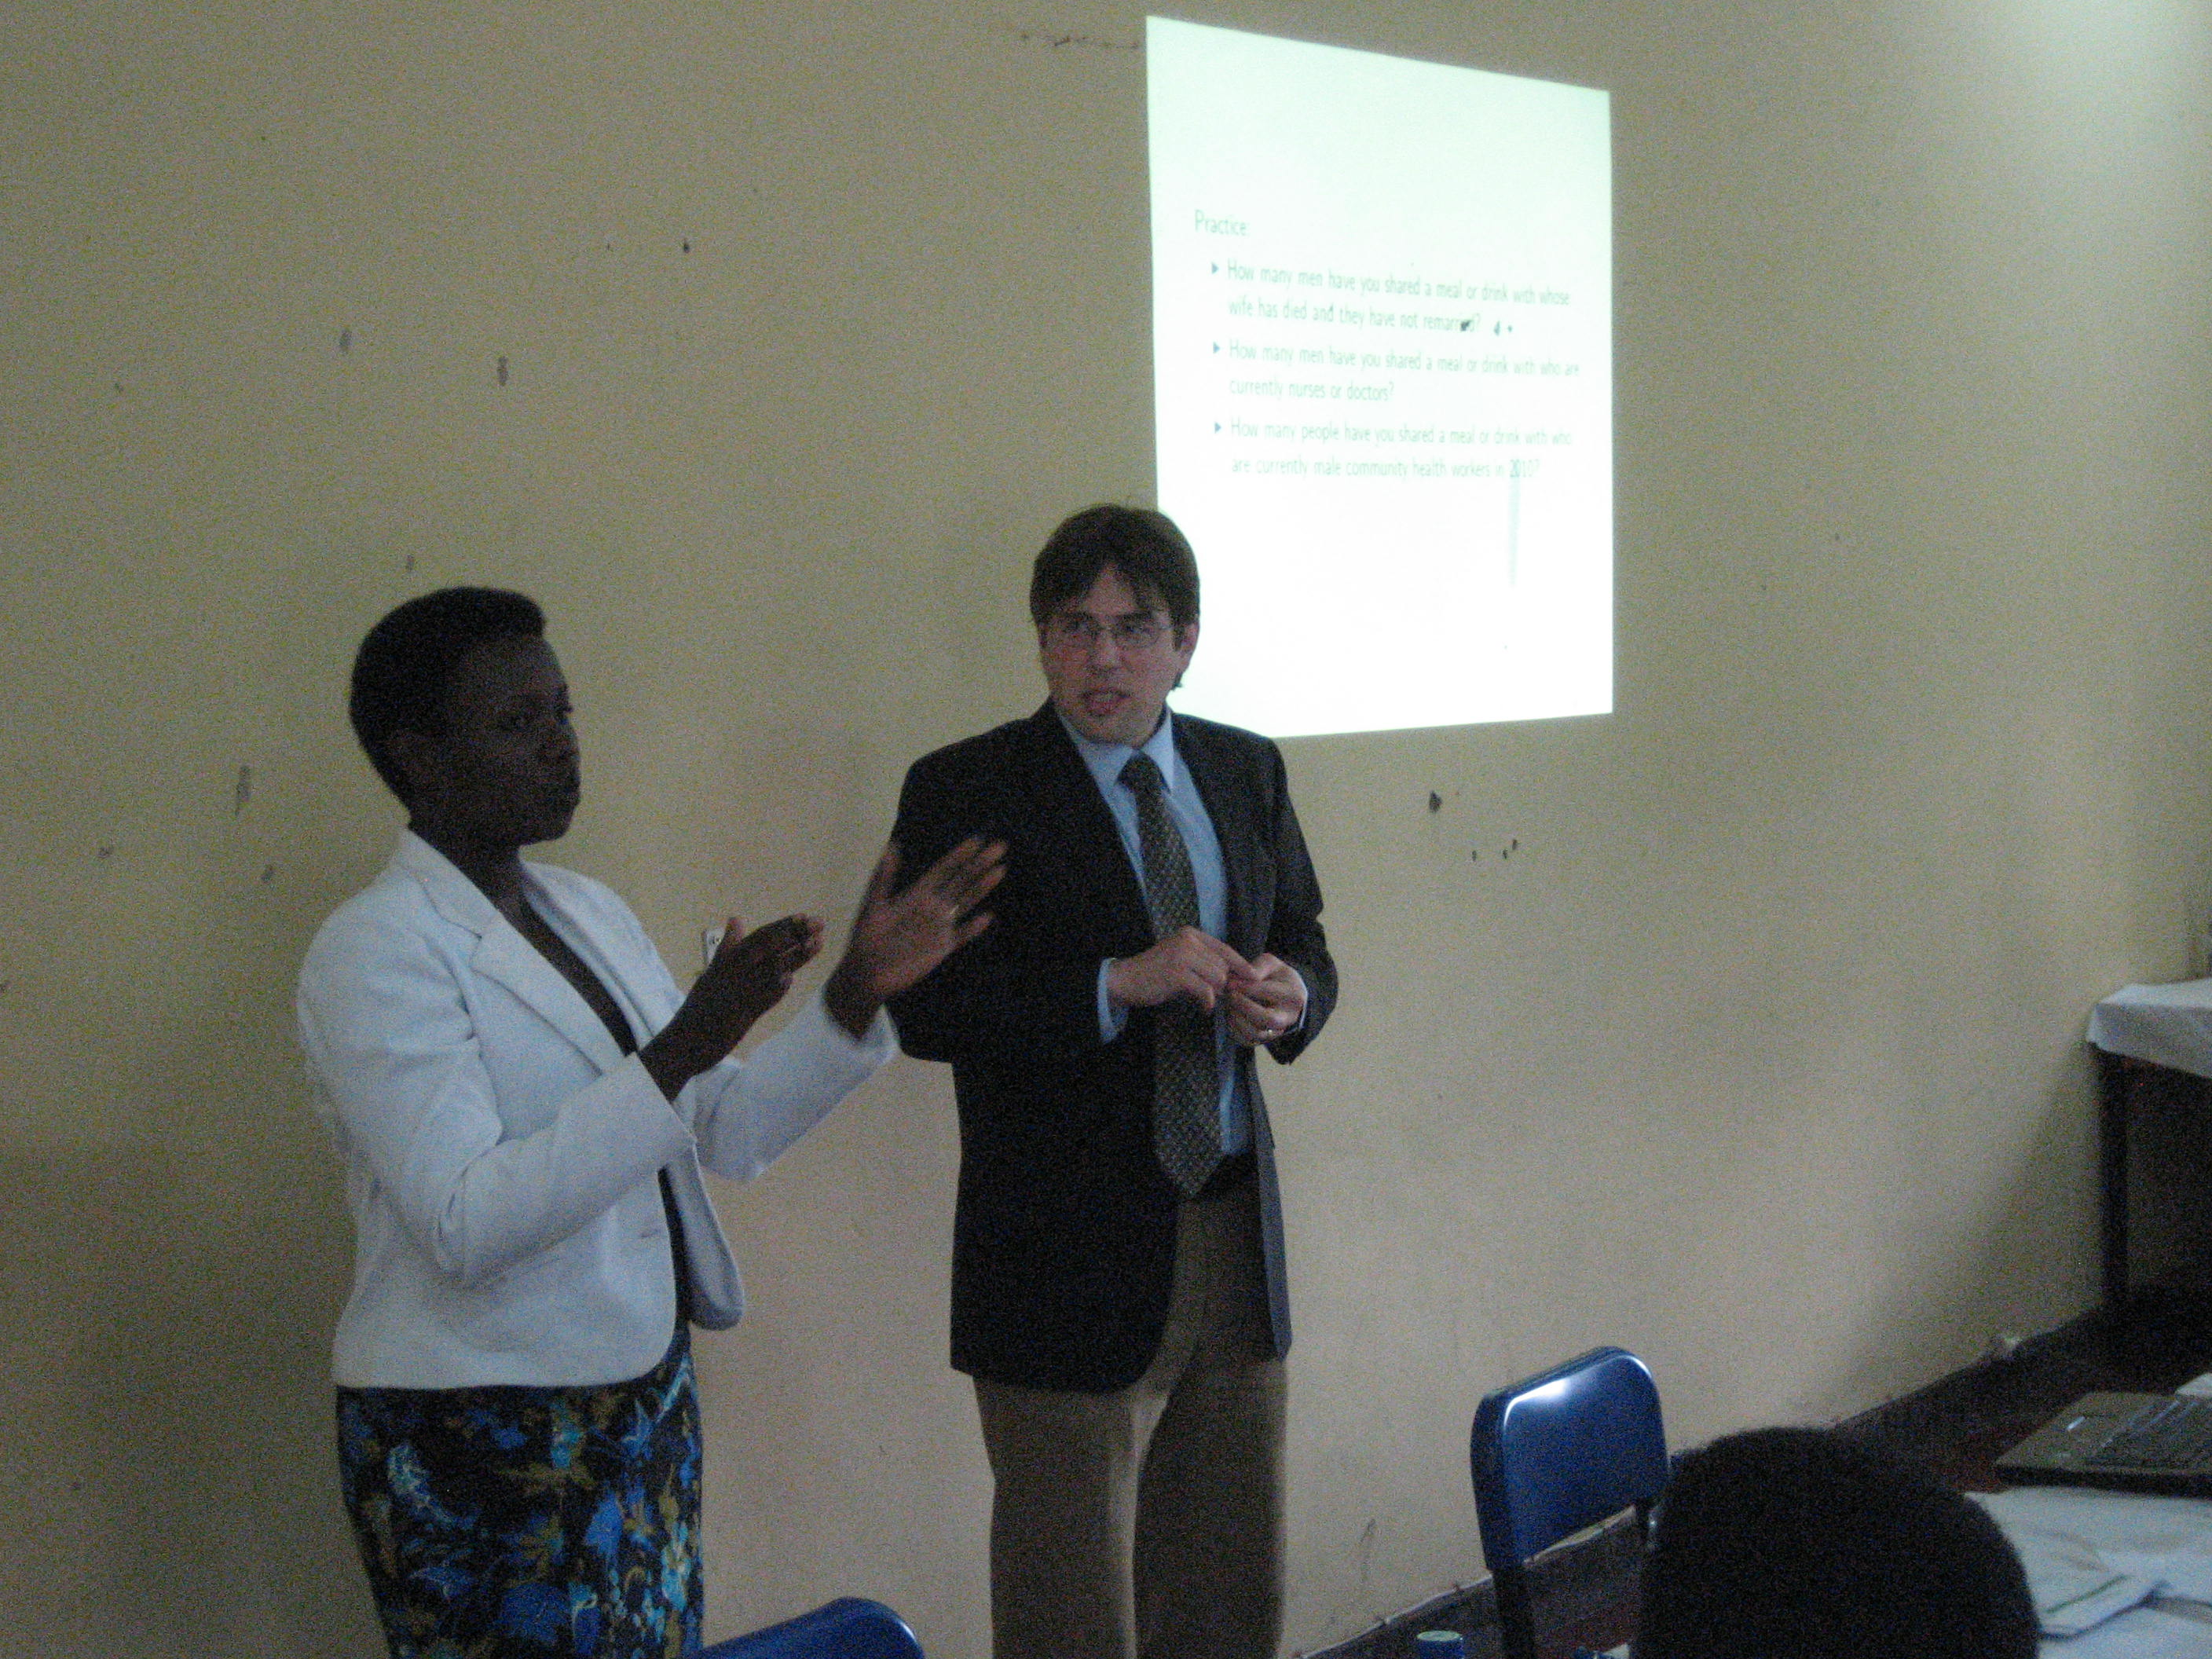
\includegraphics[width=0.8\textwidth]{figures/rwanda_matt_teaching.jpg}
\end{center}

\end{frame}
%%%%%%%%%%%%%%%%%%%%%%%%%%%
\begin{frame}

\begin{center}
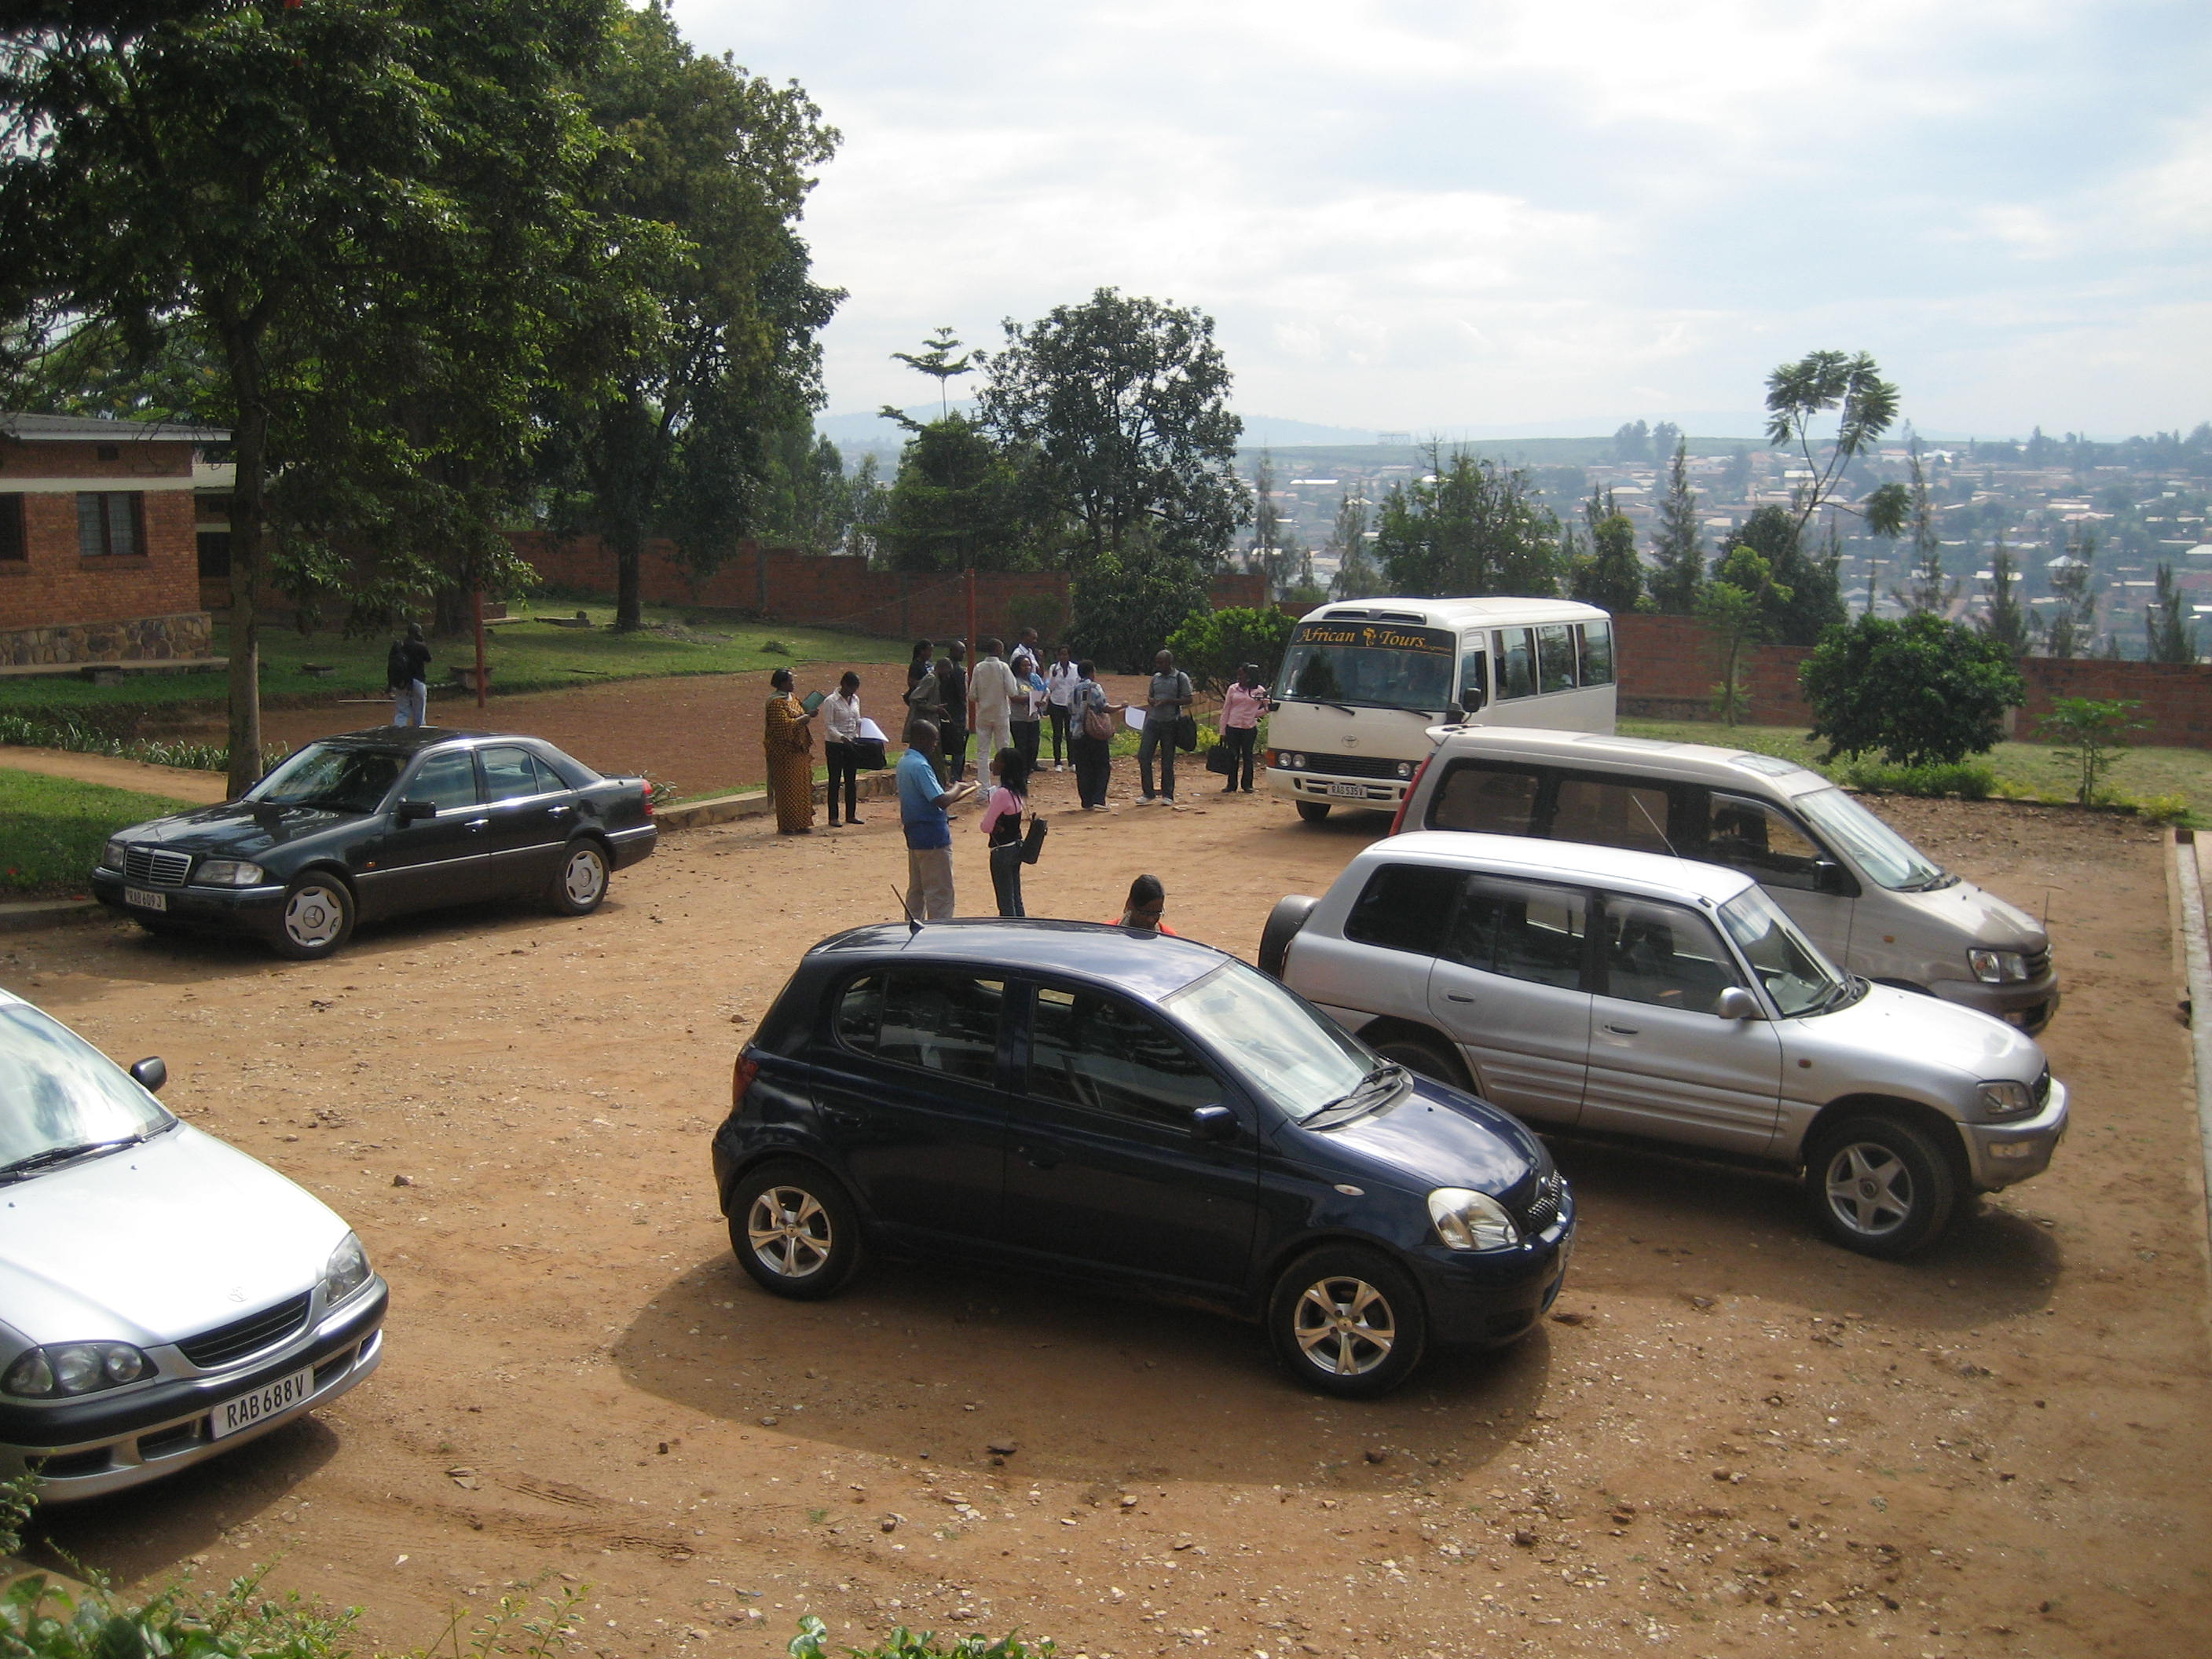
\includegraphics[width=0.8\textwidth]{figures/rwanda_interviewer_bus.jpg}
\end{center}

\end{frame}
%%%%%%%%%%%%%%%%%%%%%%%%%%%
\begin{frame}

\begin{center}
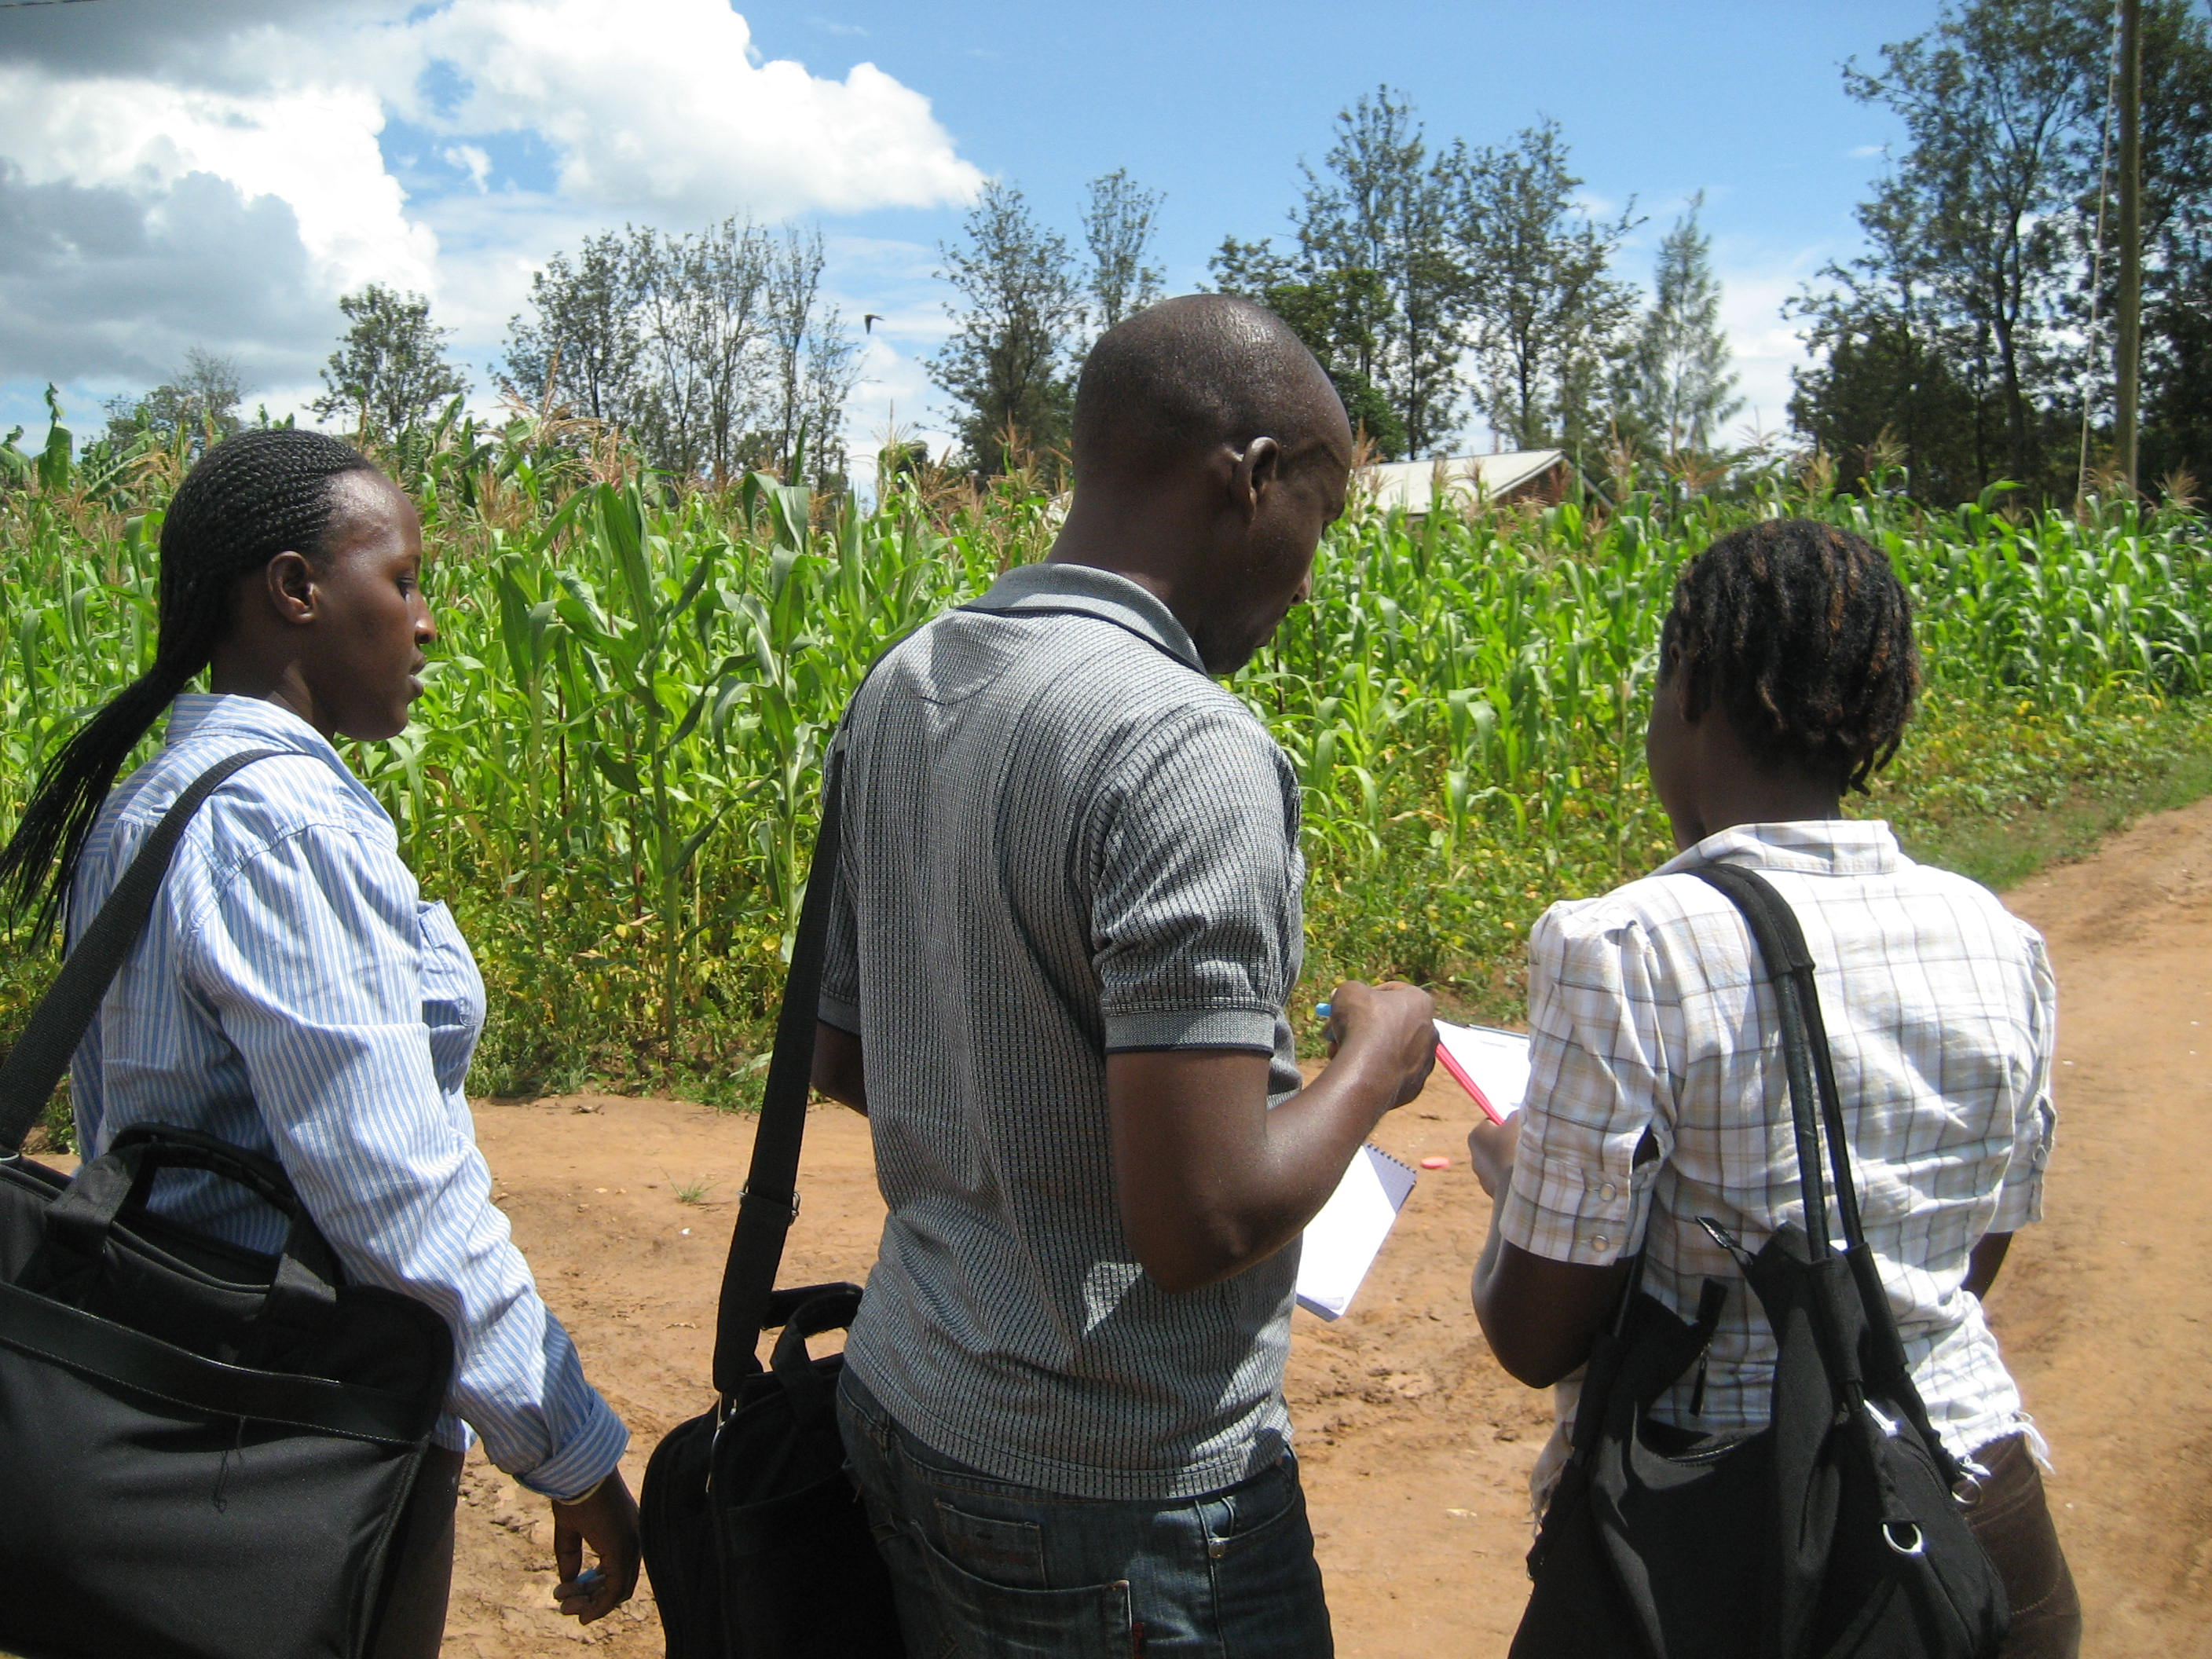
\includegraphics[width=0.8\textwidth]{figures/rwanda_fieldwork.jpg}
\end{center}

\end{frame}
%%%%%%%%%%%%%%%%%%%%%%%%%%%
\begin{frame}

\begin{center}
\includegraphics<1>[width=0.7\textwidth]{figures/tie_strength_axes}
\includegraphics<2>[width=0.7\textwidth]{figures/tie_strength_sampling}
\includegraphics<3>[width=0.7\textwidth]{figures/tie_strength_sampling_non_sampling}
\includegraphics<4>[width=0.7\textwidth]{figures/tie_strength_sampling_non_sampling_total}
\includegraphics<5>[width=0.7\textwidth]{figures/tie_strength_total}
\end{center}

\note{Think back to Granovetter}

\end{frame}
%%%%%%%%%%%%%%%%%%%%%%%%%%%
\begin{frame}
\frametitle{}

{\Large
\begin{center}
\textcolor{blue}{Basic definition} ($n=2,500$)
\end{center}
}
\begin{itemize}
\item people you know by sight and name and who also know you by sight and name  
\item people you have \textcolor{blue}{had some contact with} in the past 12 months
\item people of all ages who live in Rwanda
\end{itemize}

{\Large
\begin{center}
\textcolor{red}{Meal definition} ($n=2,500$)
\end{center}
}
\begin{itemize}
\item people you know by sight and name and who also know you by sight and name  
\item people you have \textcolor{red}{shared a meal or drink with} in the past 12 months
\item people of all ages who live in Rwanda
\end{itemize}

\end{frame}
%%%%%%%%%%%%%%%
\begin{frame}

\begin{columns}
\column{0.5\textwidth}
\begin{center}
\begin{tabular}{l}
\toprule
Priests\\
Nurses or Doctors\\
Male Community Health Worker\\
Widowers\\
Teachers\\
Divorced Men\\
Incarcerated people\\
Women who smoke\\
Muslim\\
Women who gave birth in the last 12 mo.\\
\bottomrule
\end{tabular}
\end{center}

\column{0.5\textwidth}
\begin{center}
\begin{tabular}{l}
\toprule
Twahirwa\\
Mukandekezi\\
Nyiraneza\\
Ndayambaje\\
Murekatete\\
Nsengimana\\
Mukandayisenga\\
Ndagijimana\\
Bizimana\\
Nyirahabimana\\
Nsabimana\\
Mukamana\\
\bottomrule
\end{tabular}
\end{center}

\end{columns}

\end{frame}
%%%%%%%%%%%%%%%
\begin{frame}

\begin{center}
\includegraphics<1>[width=0.6\textwidth]{figures/rwanda_mean_reported_ties}
\end{center}

\end{frame}
%%%%%%%%%%%%%%%
\begin{frame}

\begin{center}
\includegraphics<1>[width=0.8\textwidth]{figures/feehan_quantity_2016_fig2}
\end{center}

\end{frame}
%%%%%%%%%%%%%%%
\begin{frame}

\begin{center}
\includegraphics<1>[width=0.8\textwidth]{figures/rwanda_iv_results}
\end{center}

\begin{center}
Meal definition has lower error (RMSE, MAE, MRE)
\end{center}

\end{frame}
%%%%%%%%%%%%%%%
\begin{comment}
\begin{frame}

\begin{center}
Meal definition has lower error than basic definition
\end{center}
\vfill
\includegraphics<1>[width=\textwidth]{figures/rwanda_error_metrics}

\end{frame}
\end{comment}
%%%%%%%%%%%%%%%
\begin{frame}

\begin{center}
\includegraphics<1>[width=0.8\textwidth]{figures/rwanda_estimates_noblended}
\end{center}

\end{frame}
%%%%%%%%%%%%%%%
\begin{frame}

\begin{equation*}
\hat{N}_H  = w \cdot \hat{N}_{H [meal]} + (1 - w) \cdot \hat{N}_{H [basic]}
\end{equation*}
\pause
\vfill
\begin{equation*}
w = \frac{\widehat{\sigma}^2_{basic}}{\widehat{\sigma}^2_{basic} + \widehat{\sigma}^2_{meal}} 
\end{equation*}

\end{frame}
%%%%%%%%%%%%%%%
\begin{frame}

\begin{center}
\includegraphics<1>[width=\textwidth]{figures/rwanda_estimates_blended}
\end{center}

\end{frame}
%%%%%%%%%%%%%%%
\begin{frame}

\begin{equation*}
N_H = \alpha \hat{N}_H
\end{equation*}

where
\begin{equation*}
\alpha =  \underbrace{\left( \frac{\eta_F}{\tau_F} \right)}_{\text{reporting  distortions}} \times \underbrace{\left( \frac{1}{\phi_F \delta_F} \right)}_{\text{structural distortions}}
\end{equation*}

\end{frame}
%%%%%%%%%%%%%%%
\begin{frame}

\begin{center}
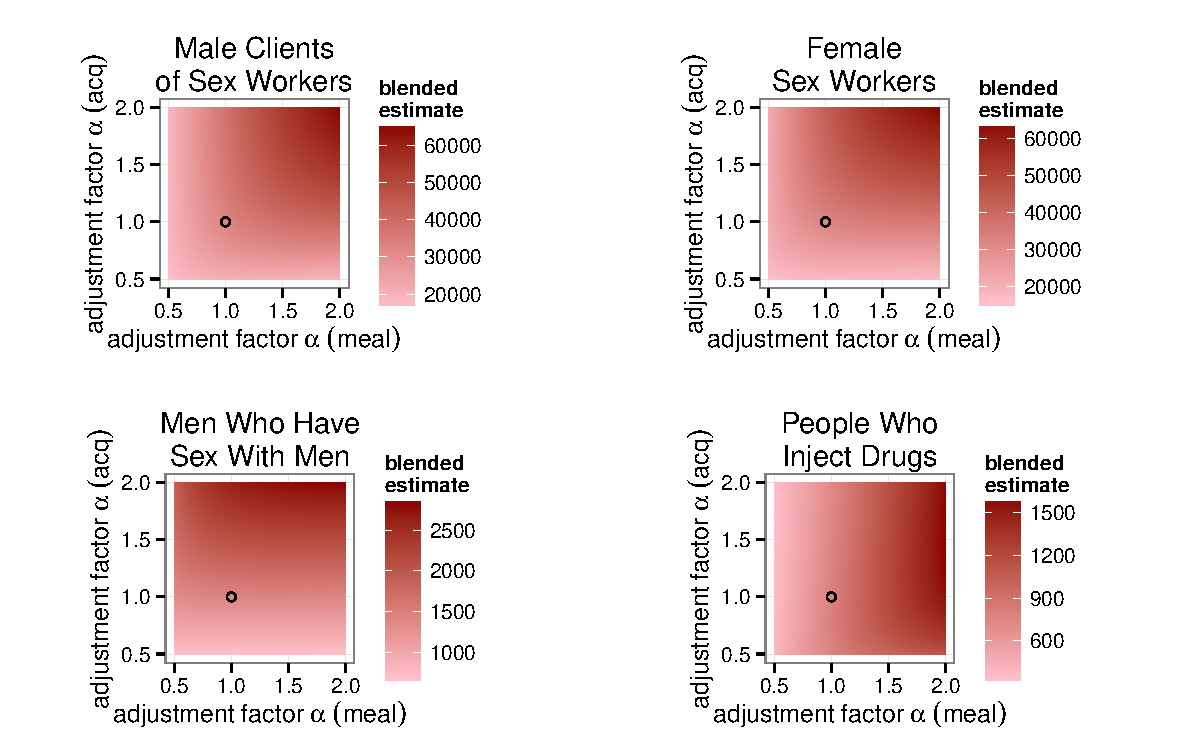
\includegraphics[width=\textwidth]{figures/feehan_quality_fig6}
\end{center}

\end{frame}
%%%%%%%%%%%%%%%
\begin{frame}

\begin{center}
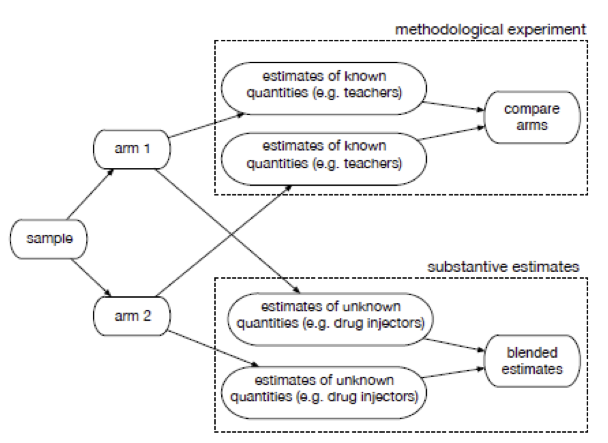
\includegraphics[width=0.8\textwidth]{figures/feehan_quality_2015_fig7}
\end{center}

\end{frame}
%%%%%%%%%%%%%%%%%%%%%%%%%%%
\begin{frame}

\LARGE{Next steps for network scale-up method}

\end{frame}
%%%%%%%%%%%%%%%%%%%%%%%%%%%
\begin{frame}

With only two arms, we cannot demonstrate U-shaped relationship!

\begin{center}
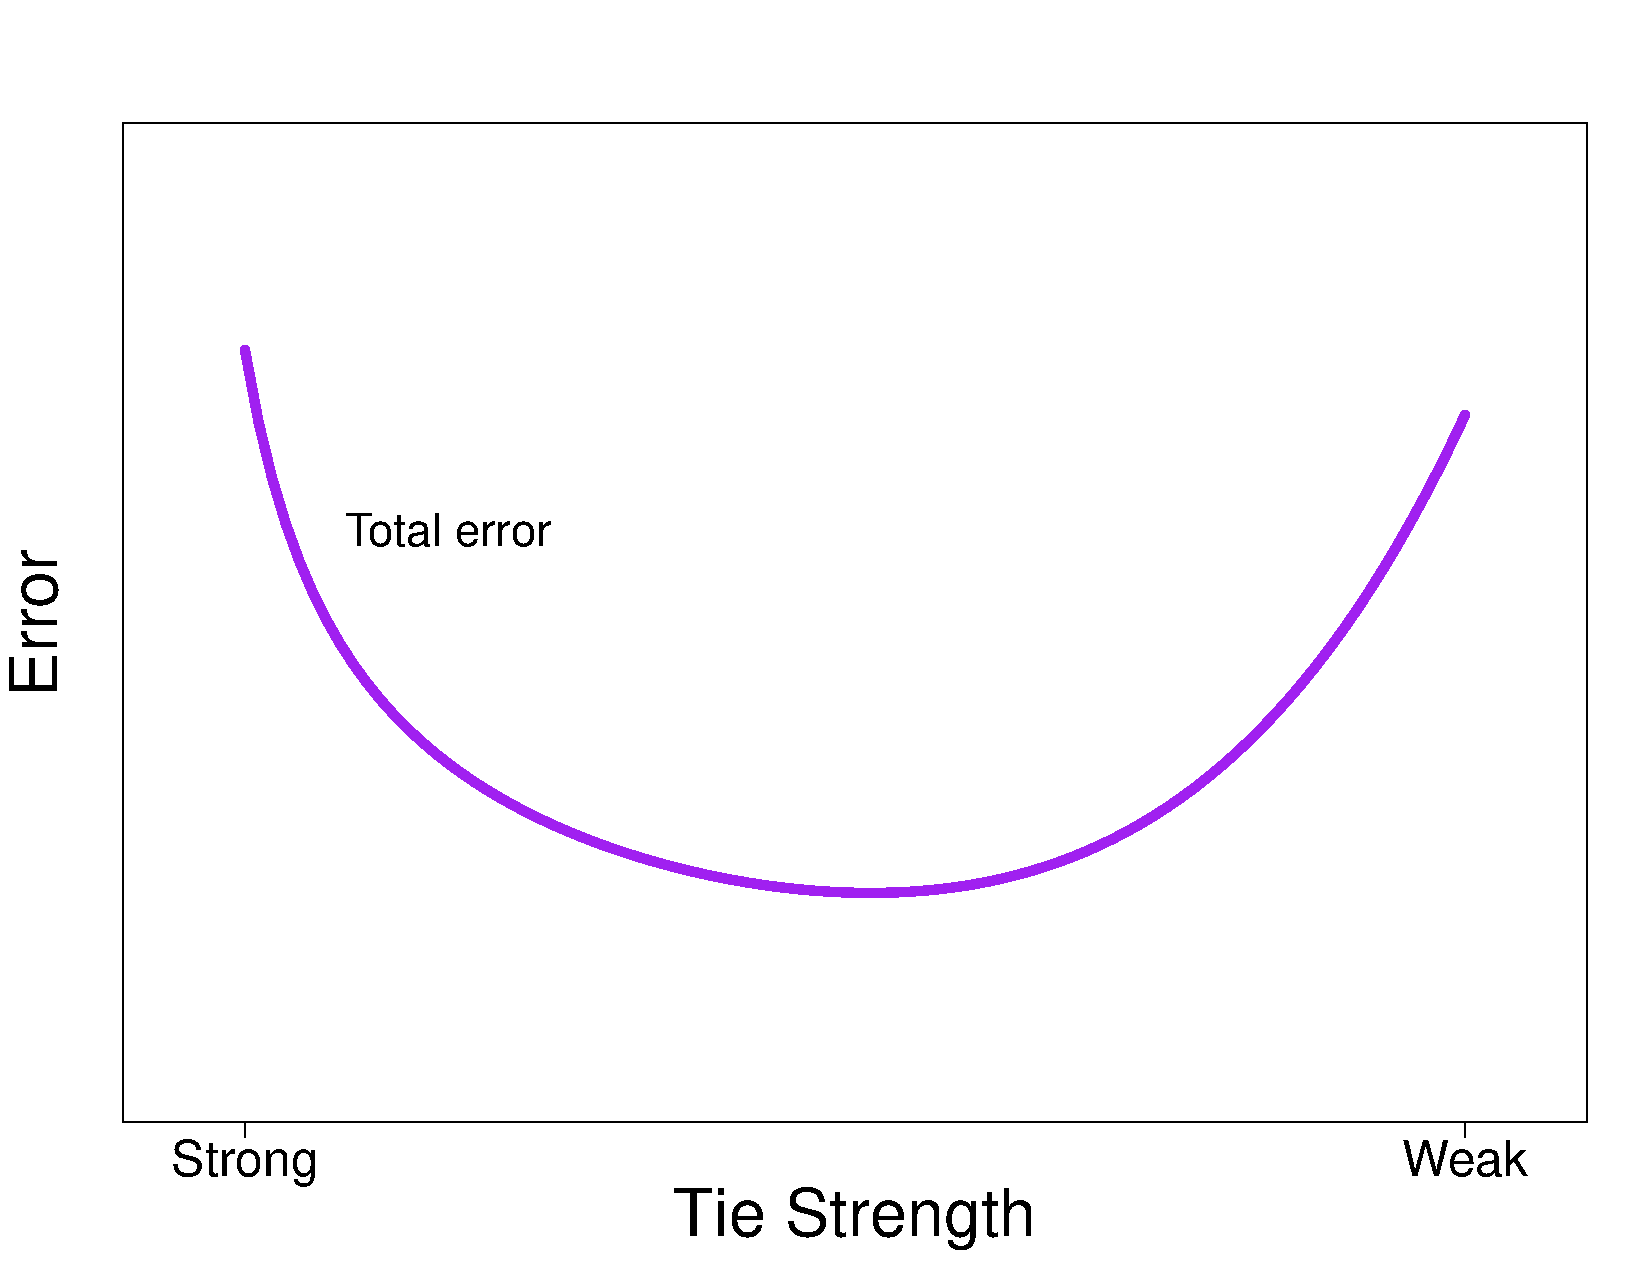
\includegraphics[width=0.25\textwidth]{figures/tie_strength_total}
\end{center}

\pause
In previous classes, we tried a survey experiment as a homework assignment in this class.  
\begin{itemize}
\item We wanted to estimate number of people dating someone from their high school and number of people dating someone from Rutgers.
\item We asked about connections to 9 groups of known size (e.g., sociology majors).
\item We used 4 definitions of to know:
\begin{enumerate}
\item shared a meal with yesterday
\item shared a meal with in the past seven days
\item shared a meal with this semester
\item shared a meal with this academic year
\end{enumerate}
\end{itemize}

\end{frame}
%%%%%%%%%%%%%%%%%%%%%%%%%%
\begin{frame}

\begin{center}
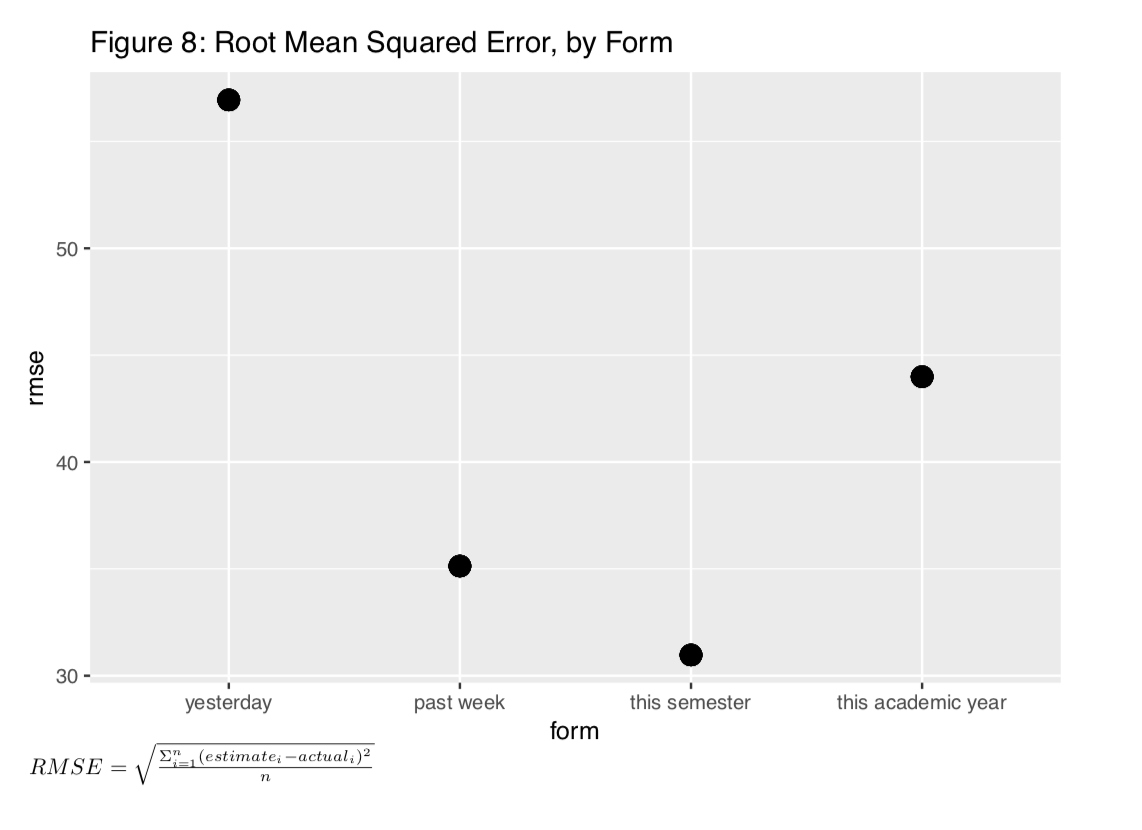
\includegraphics[width=0.7\textwidth]{figures/soc204_s2017_assignment8_mse_ushape}
\end{center}

\end{frame}
%%%%%%%%%%%%%%%%%%%%%%%%%%
\begin{frame}

\begin{center}
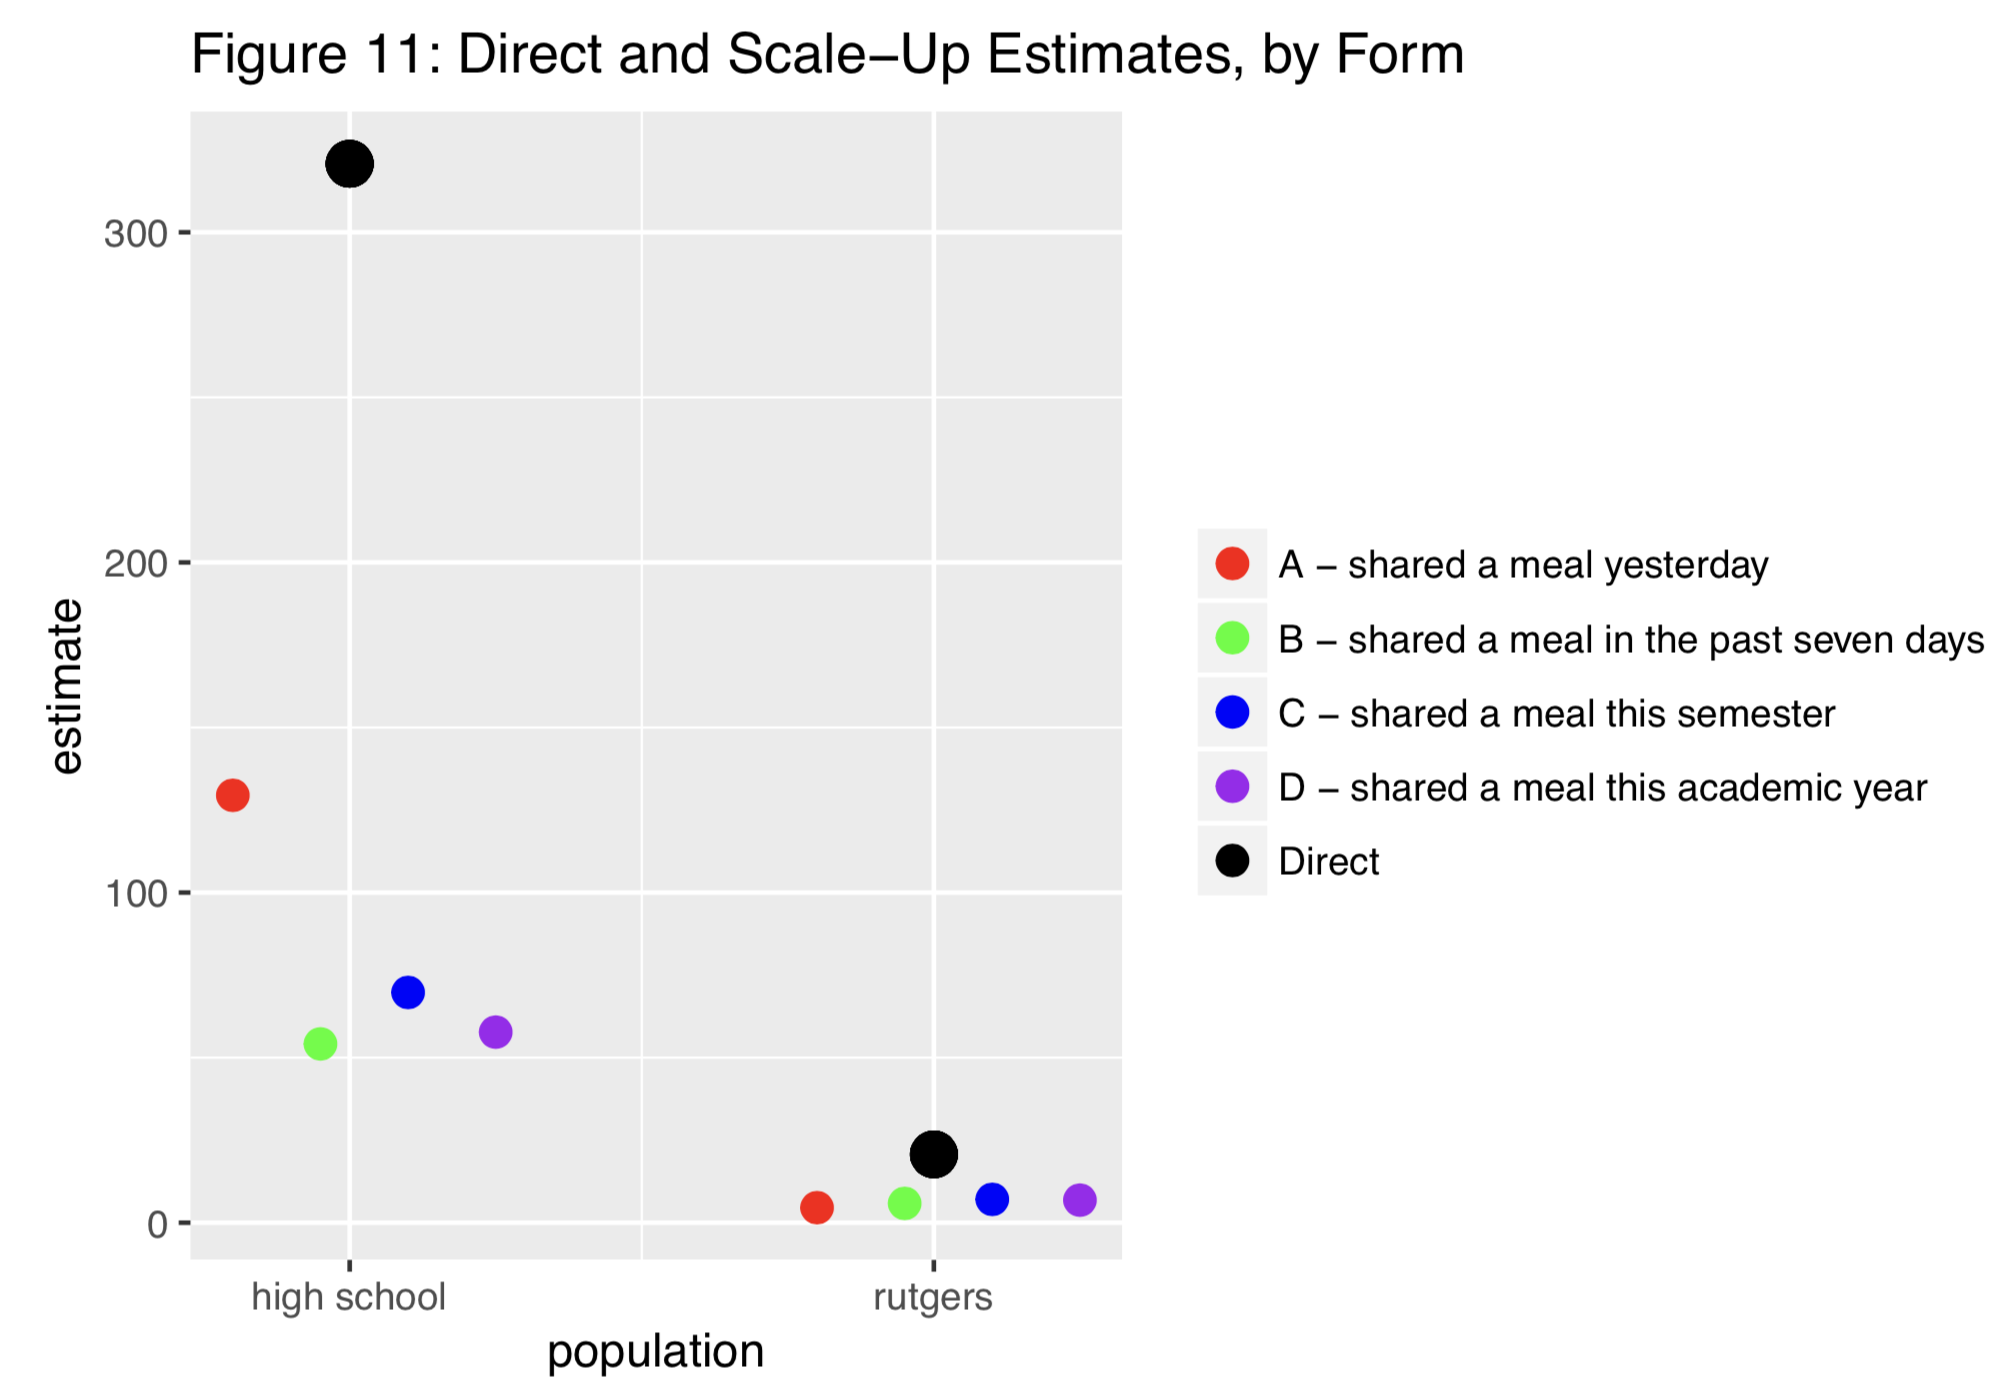
\includegraphics[width=0.7\textwidth]{figures/soc204_s2017_assignment8_estimates}
\end{center}

\begin{itemize}
\item scale-up estimates might be too low because of imperfect visibility
\end{itemize}


\end{frame}
%%%%%%%%%%%%%%%%%%%%%%%%%%
\begin{frame}

Lecture 23: Who knows what about who?
\begin{itemize}
\item Salganik, M.J. et al. (2011). The game of contacts: Estimating the social visibility of groups. \textit{Social Networks}.
\item Cowan, S. (2014). Secrets and Misperceptions: The Creation of Self-Fulfilling Illusions. \textit{Sociological Science}.
\end{itemize}

\end{frame}
%%%%%%%%%%%%%%%%%%%%%%%%%%


\end{document}
